This section provides a full overview of the training and evaluation results of the agents in the two-player self-play setting. The training and evaluation results are presented in the form of the average score and loss curves for each agent during training. The training and loss curves provide insights into the learning process of the agents and their performance in the game and are presented in Figures ~\ref{fig:dqnmean} - ~\ref{fig:sad3loss}.

We observe that the simple DQN agent struggles to learn the game effectively and fails to achieve a high score in the game. The agent's performance is unstable, and it fails to maintain a high score over time, despite the loss curve showing a decreasing trend. The agent's performance is likely limited by the simple DQN architecture and the sample-limited training setting. The agent's performance is presented in Figures ~\ref{fig:dqnmean} and ~\ref{fig:dqnloss}.

All of the Rainbow agents show the highest performance in the game, with the base Rainbow agent achieving the highest average score. The Rainbow agents show a cyclic pattern of improvement and regression in their performance, discussed earlier in Section ~\ref{sec:results}. Interestingly, the Rainbow agents with a 3-step and 5-step history show no clear trend in their loss curves, despite showing a general improvement in their performance over time. This is only present in the Rainbow agents, and it is likely due to the added noise from the Noisy Networks exploration strategy in combination with the larger history lengths causing some instability in the learning process. It is also likely linked to the cyclic pattern of improvement and regression in the Rainbow agents' performance. The Rainbow agents' performance is presented in Figures ~\ref{fig:rainbowmean} - ~\ref{fig:rainbow5loss}.

Both the SAD and Distributed agents show a very pronounced rapid increase in loss for the first 10-20 episodes, followed by a rapid decrease in loss. This can likely be explained by the lack of meaningful experiences in the replay buffer at the start of training, leading to a high TD error and thus a high loss. As the agents gain more experience, the loss decreases rapidly, indicating that the agents are learning effectively from the experiences. Additionally, the target network would only begin to stabilize after a few episodes, leading to a decrease in the loss. This is also likely exacerbated by the initial fully random exploration coupled with Hanabi's partially observable nature. The SAD and Distributed agents' performance is presented in Figures ~\ref{fig:distributed} - ~\ref{fig:sad3loss}.

\begin{figure*}[h]
    \centering
    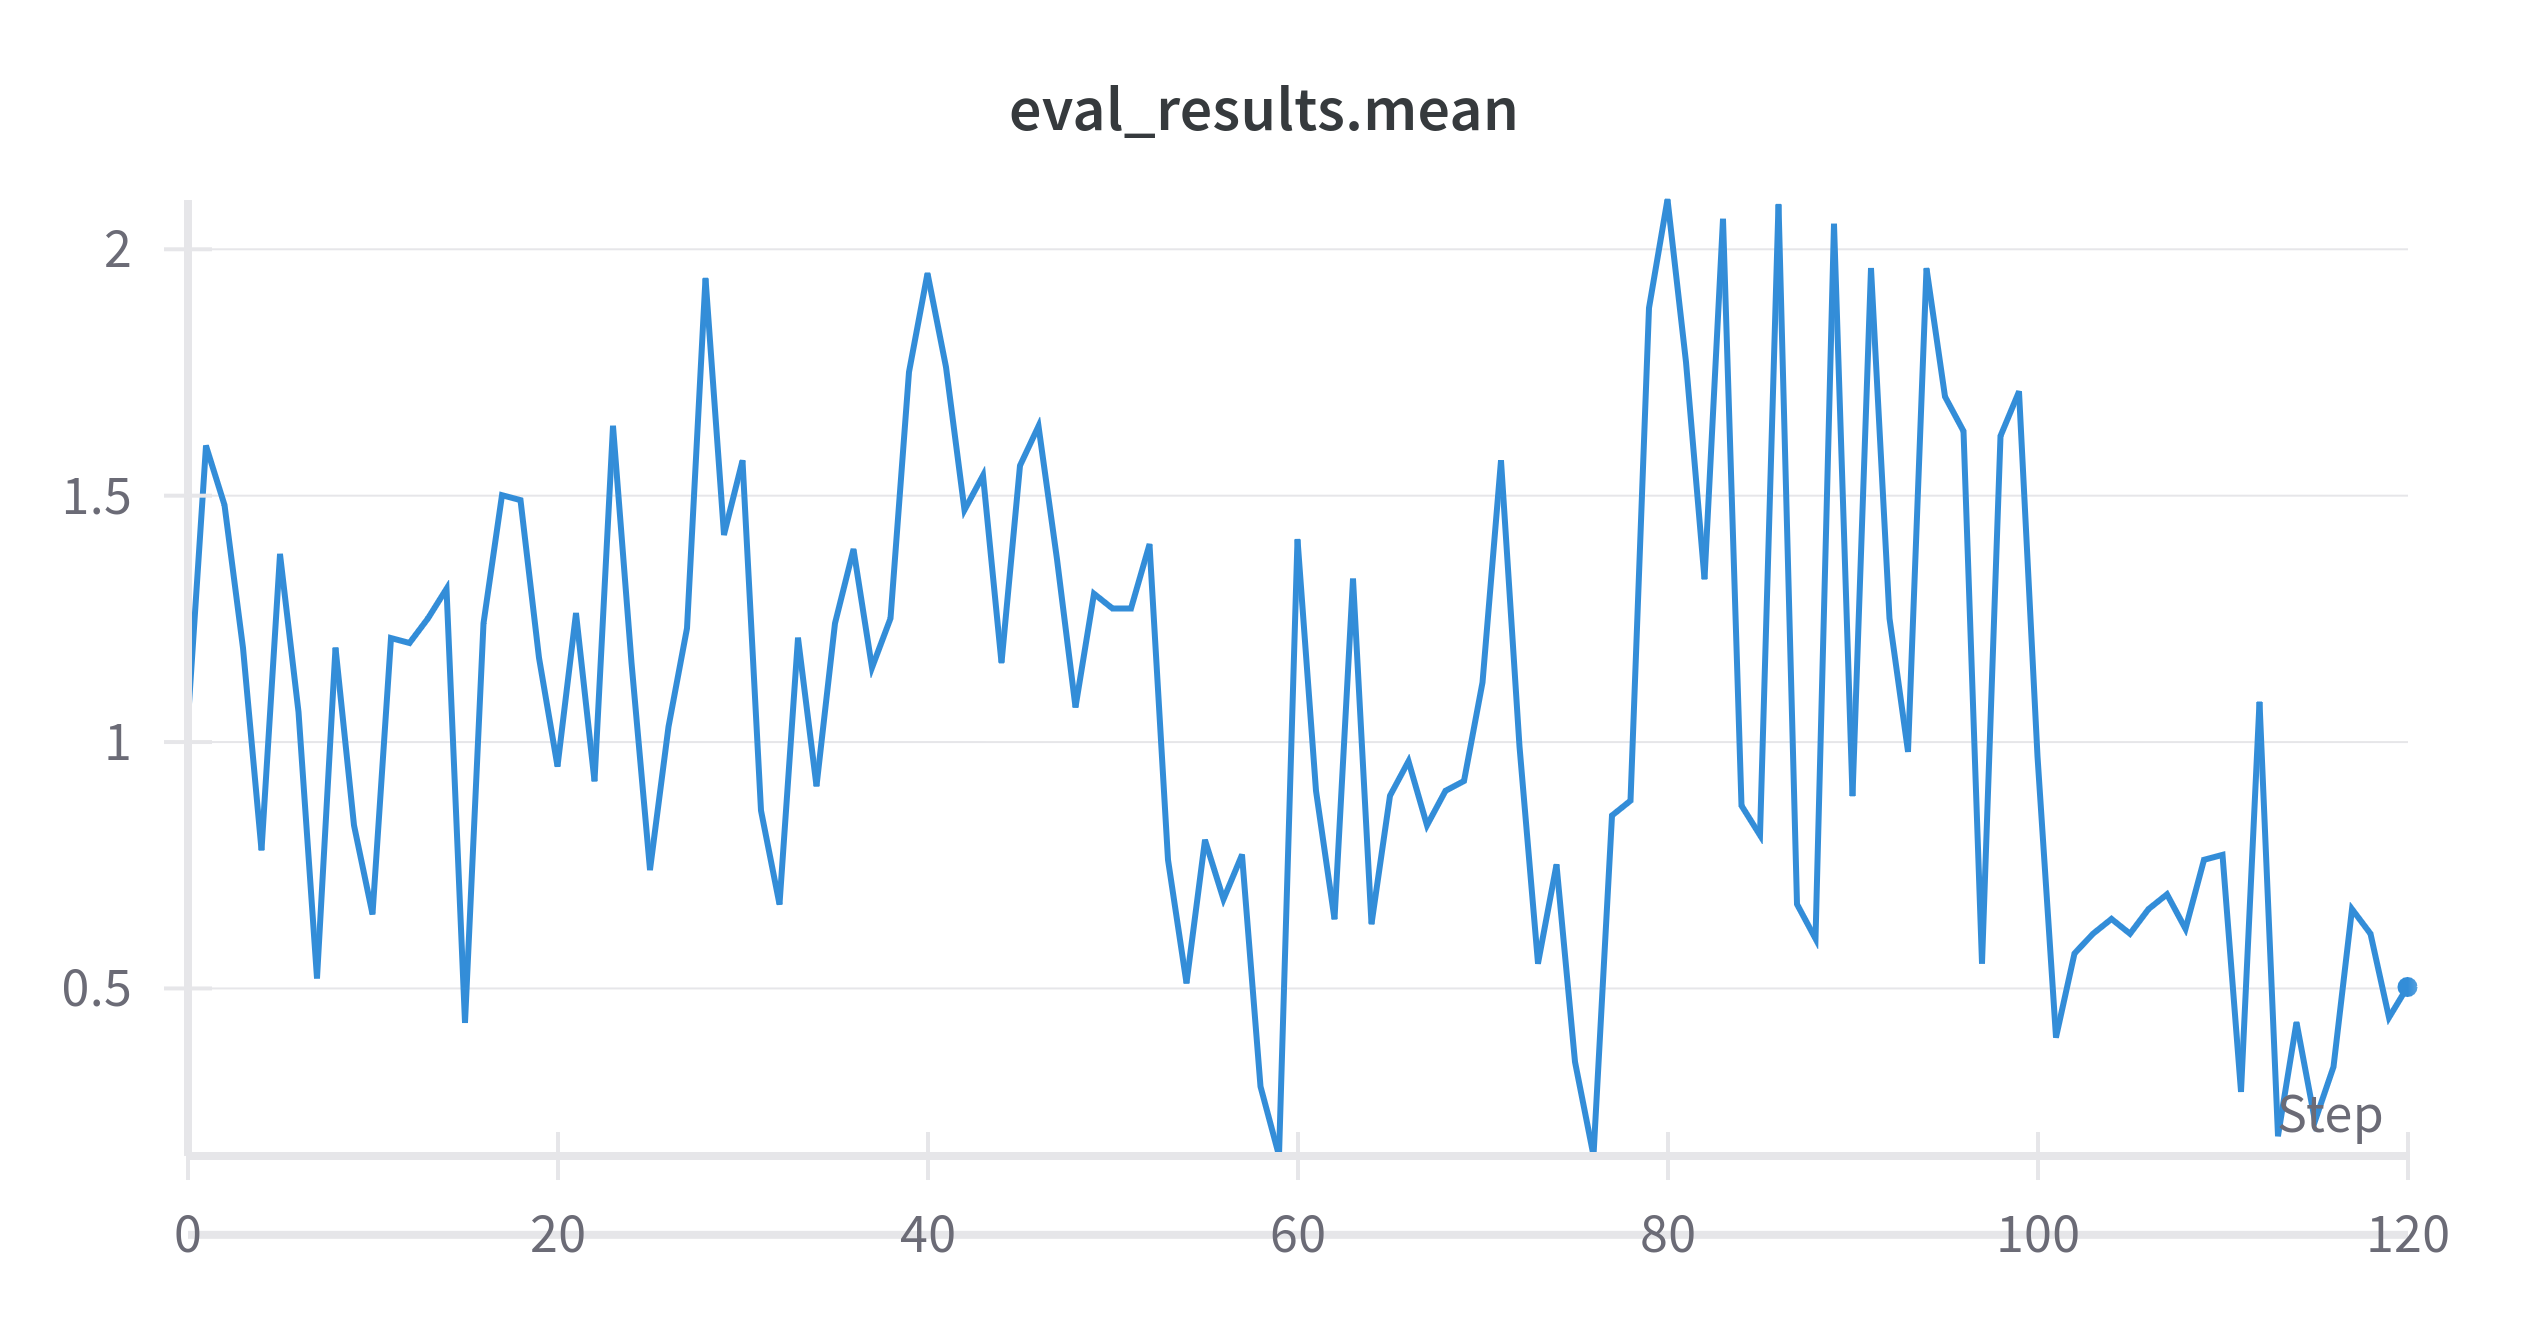
\includegraphics[width=\linewidth]{results/IQL.png}
    \caption{
      Training curve for Simple DQN Agent
    }
    \Description{Training curve for Simple DQN Agent}
    \label{fig:dqnmean}
  \end{figure*}
  
  \begin{figure*}[h]
    \centering
    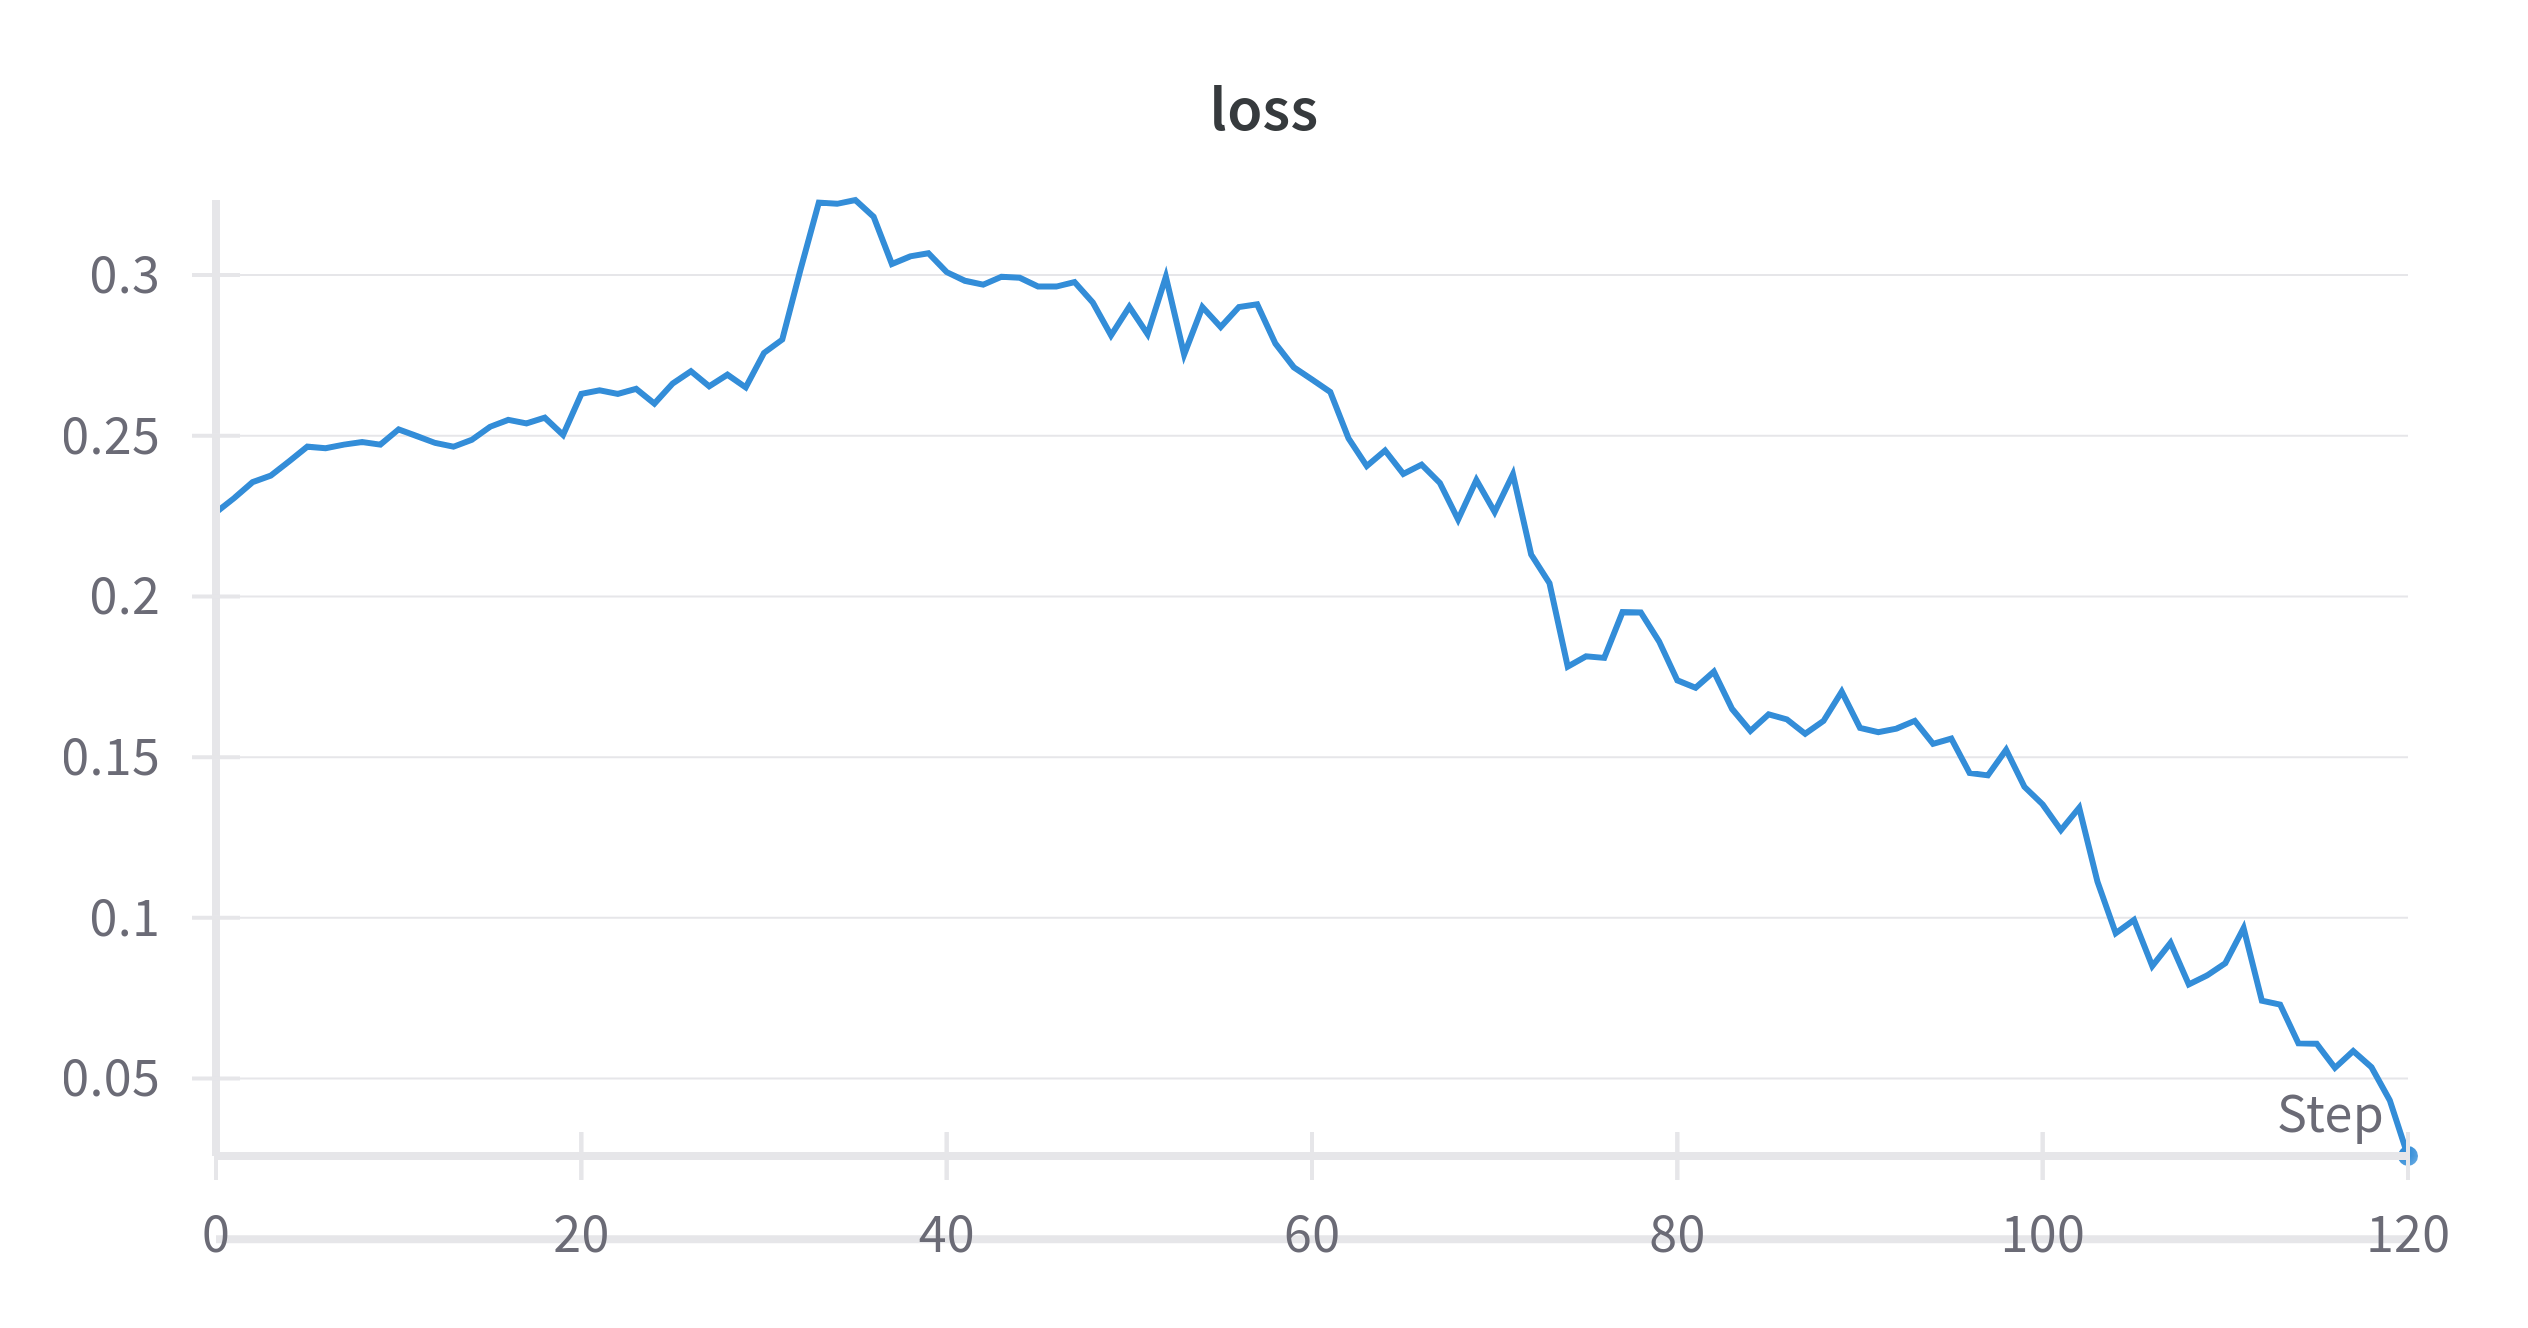
\includegraphics[width=\linewidth]{results/IQL-loss.png}
    \caption{
        Loss curve for Simple DQN Agent
    }
    \Description{Loss curve for Simple DQN Agent}
    \label{fig:dqnloss}
  \end{figure*}



  \begin{figure*}[h]
    \centering
    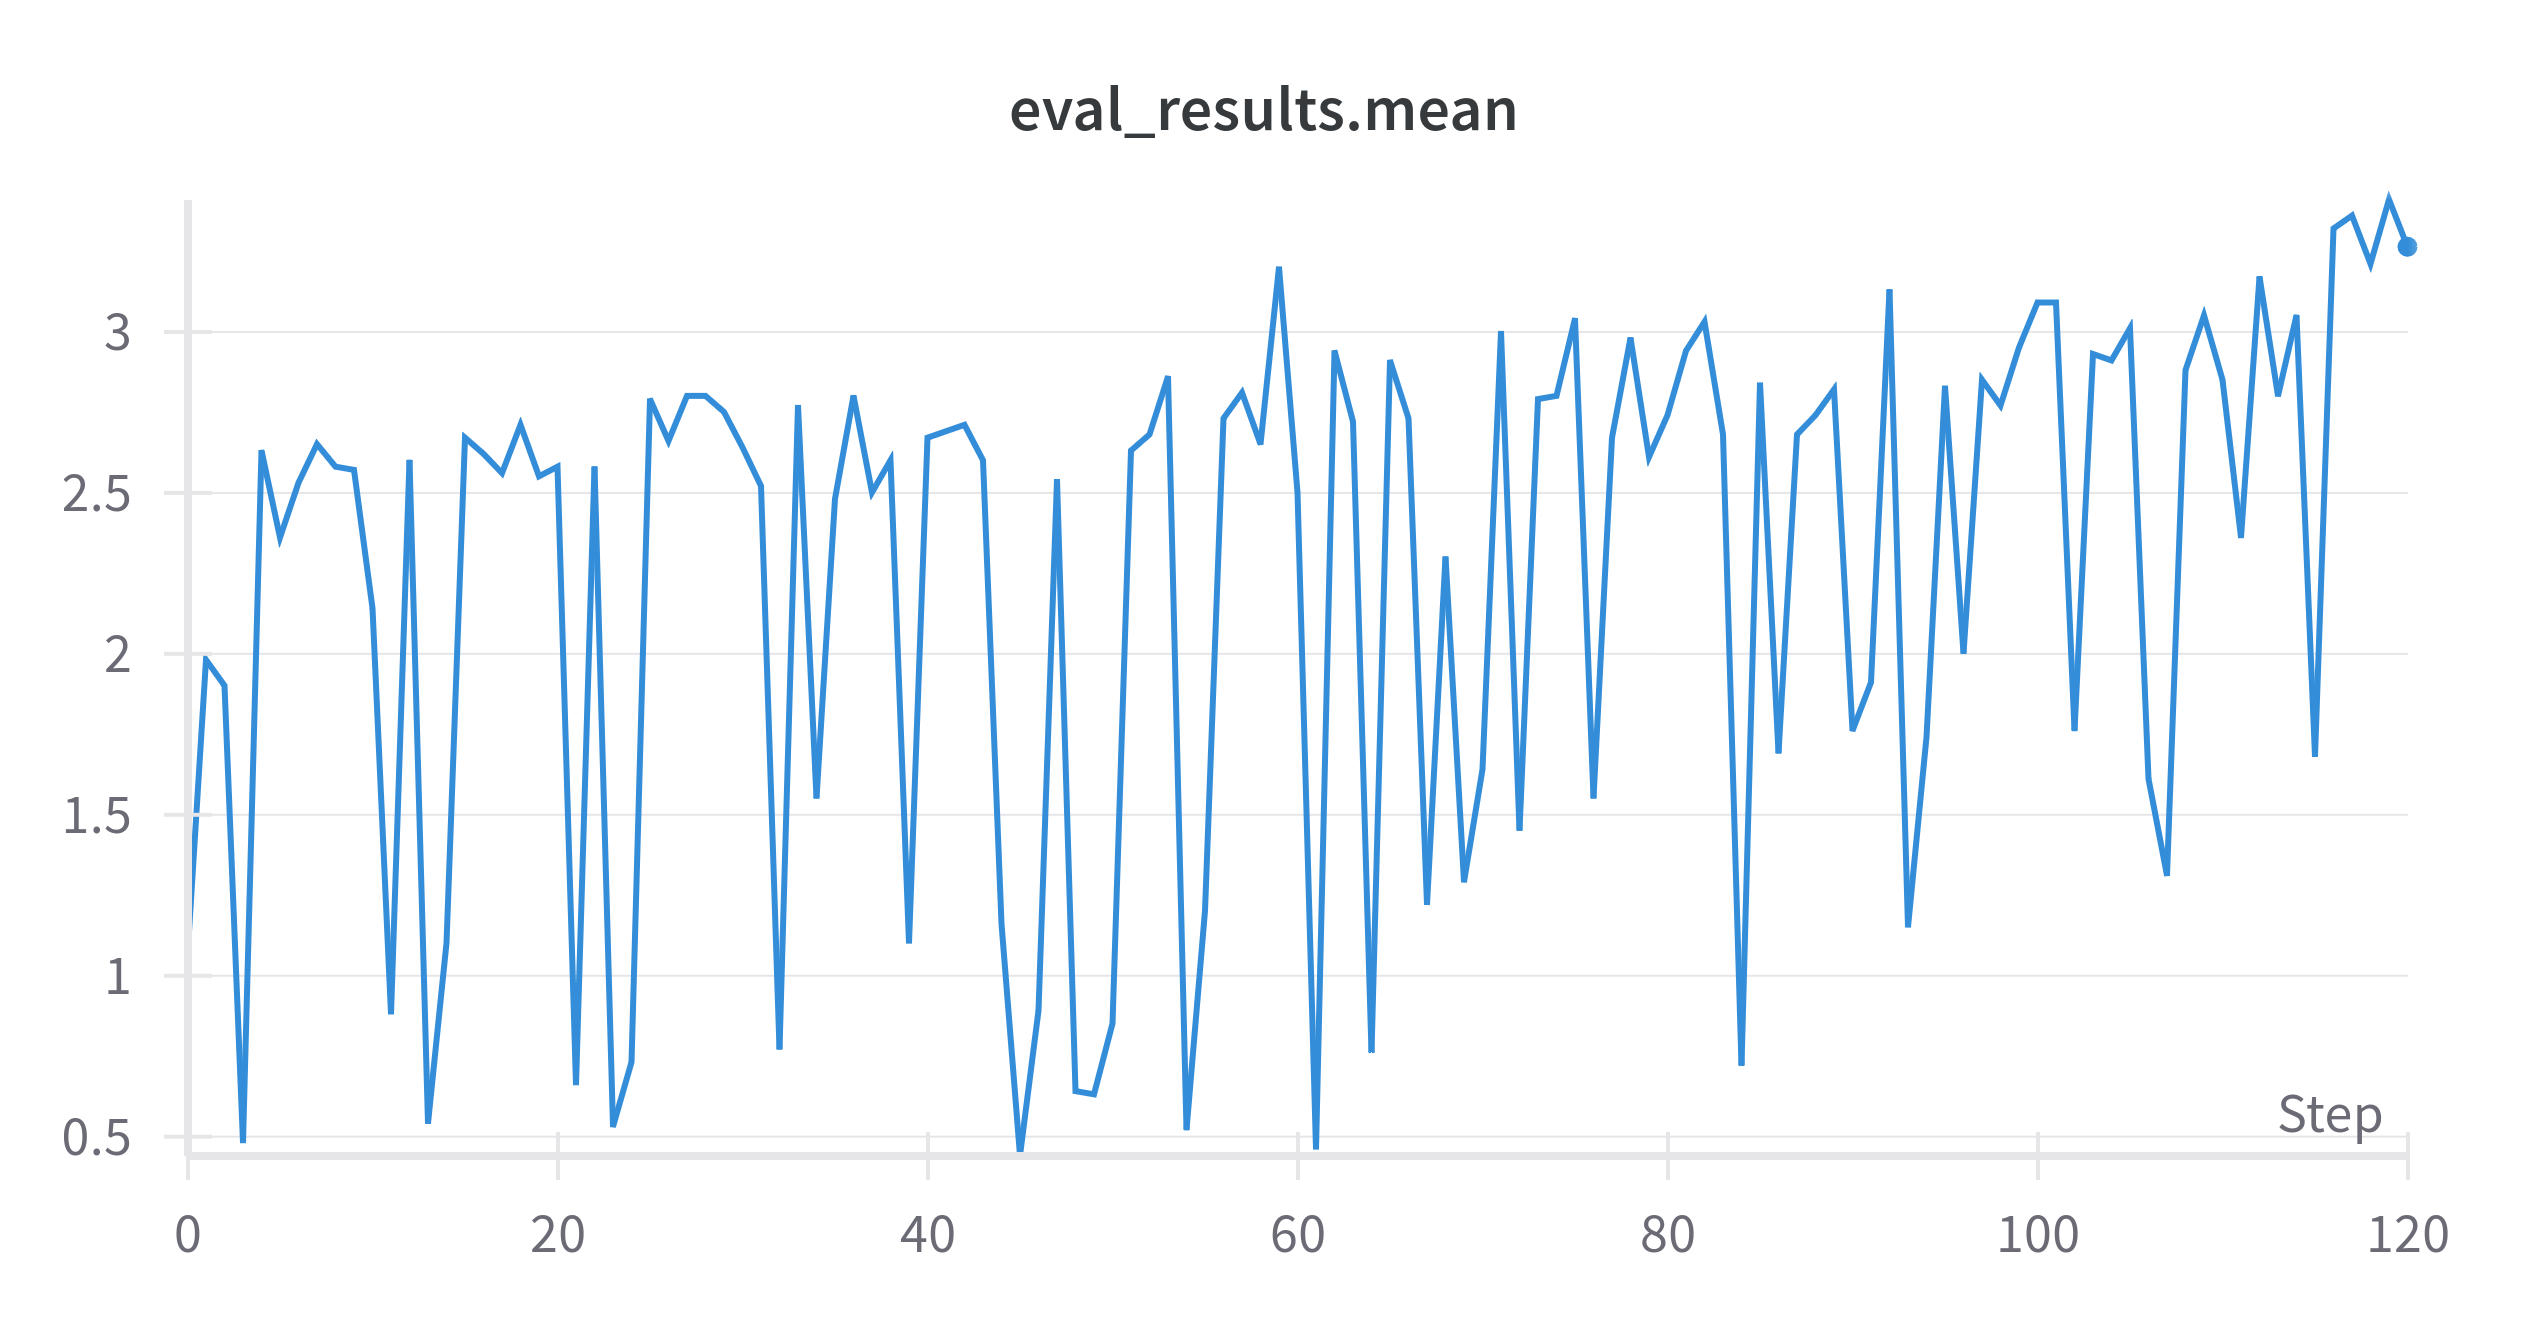
\includegraphics[width=\linewidth]{results/RAINBOW-mean.png}
    \caption{
      Training curve for Rainbow Agent
    }
    \Description{Training curve for Rainbow Agent}
    \label{fig:rainbowmean}
  \end{figure*}
  \begin{figure*}[h]
    \centering
    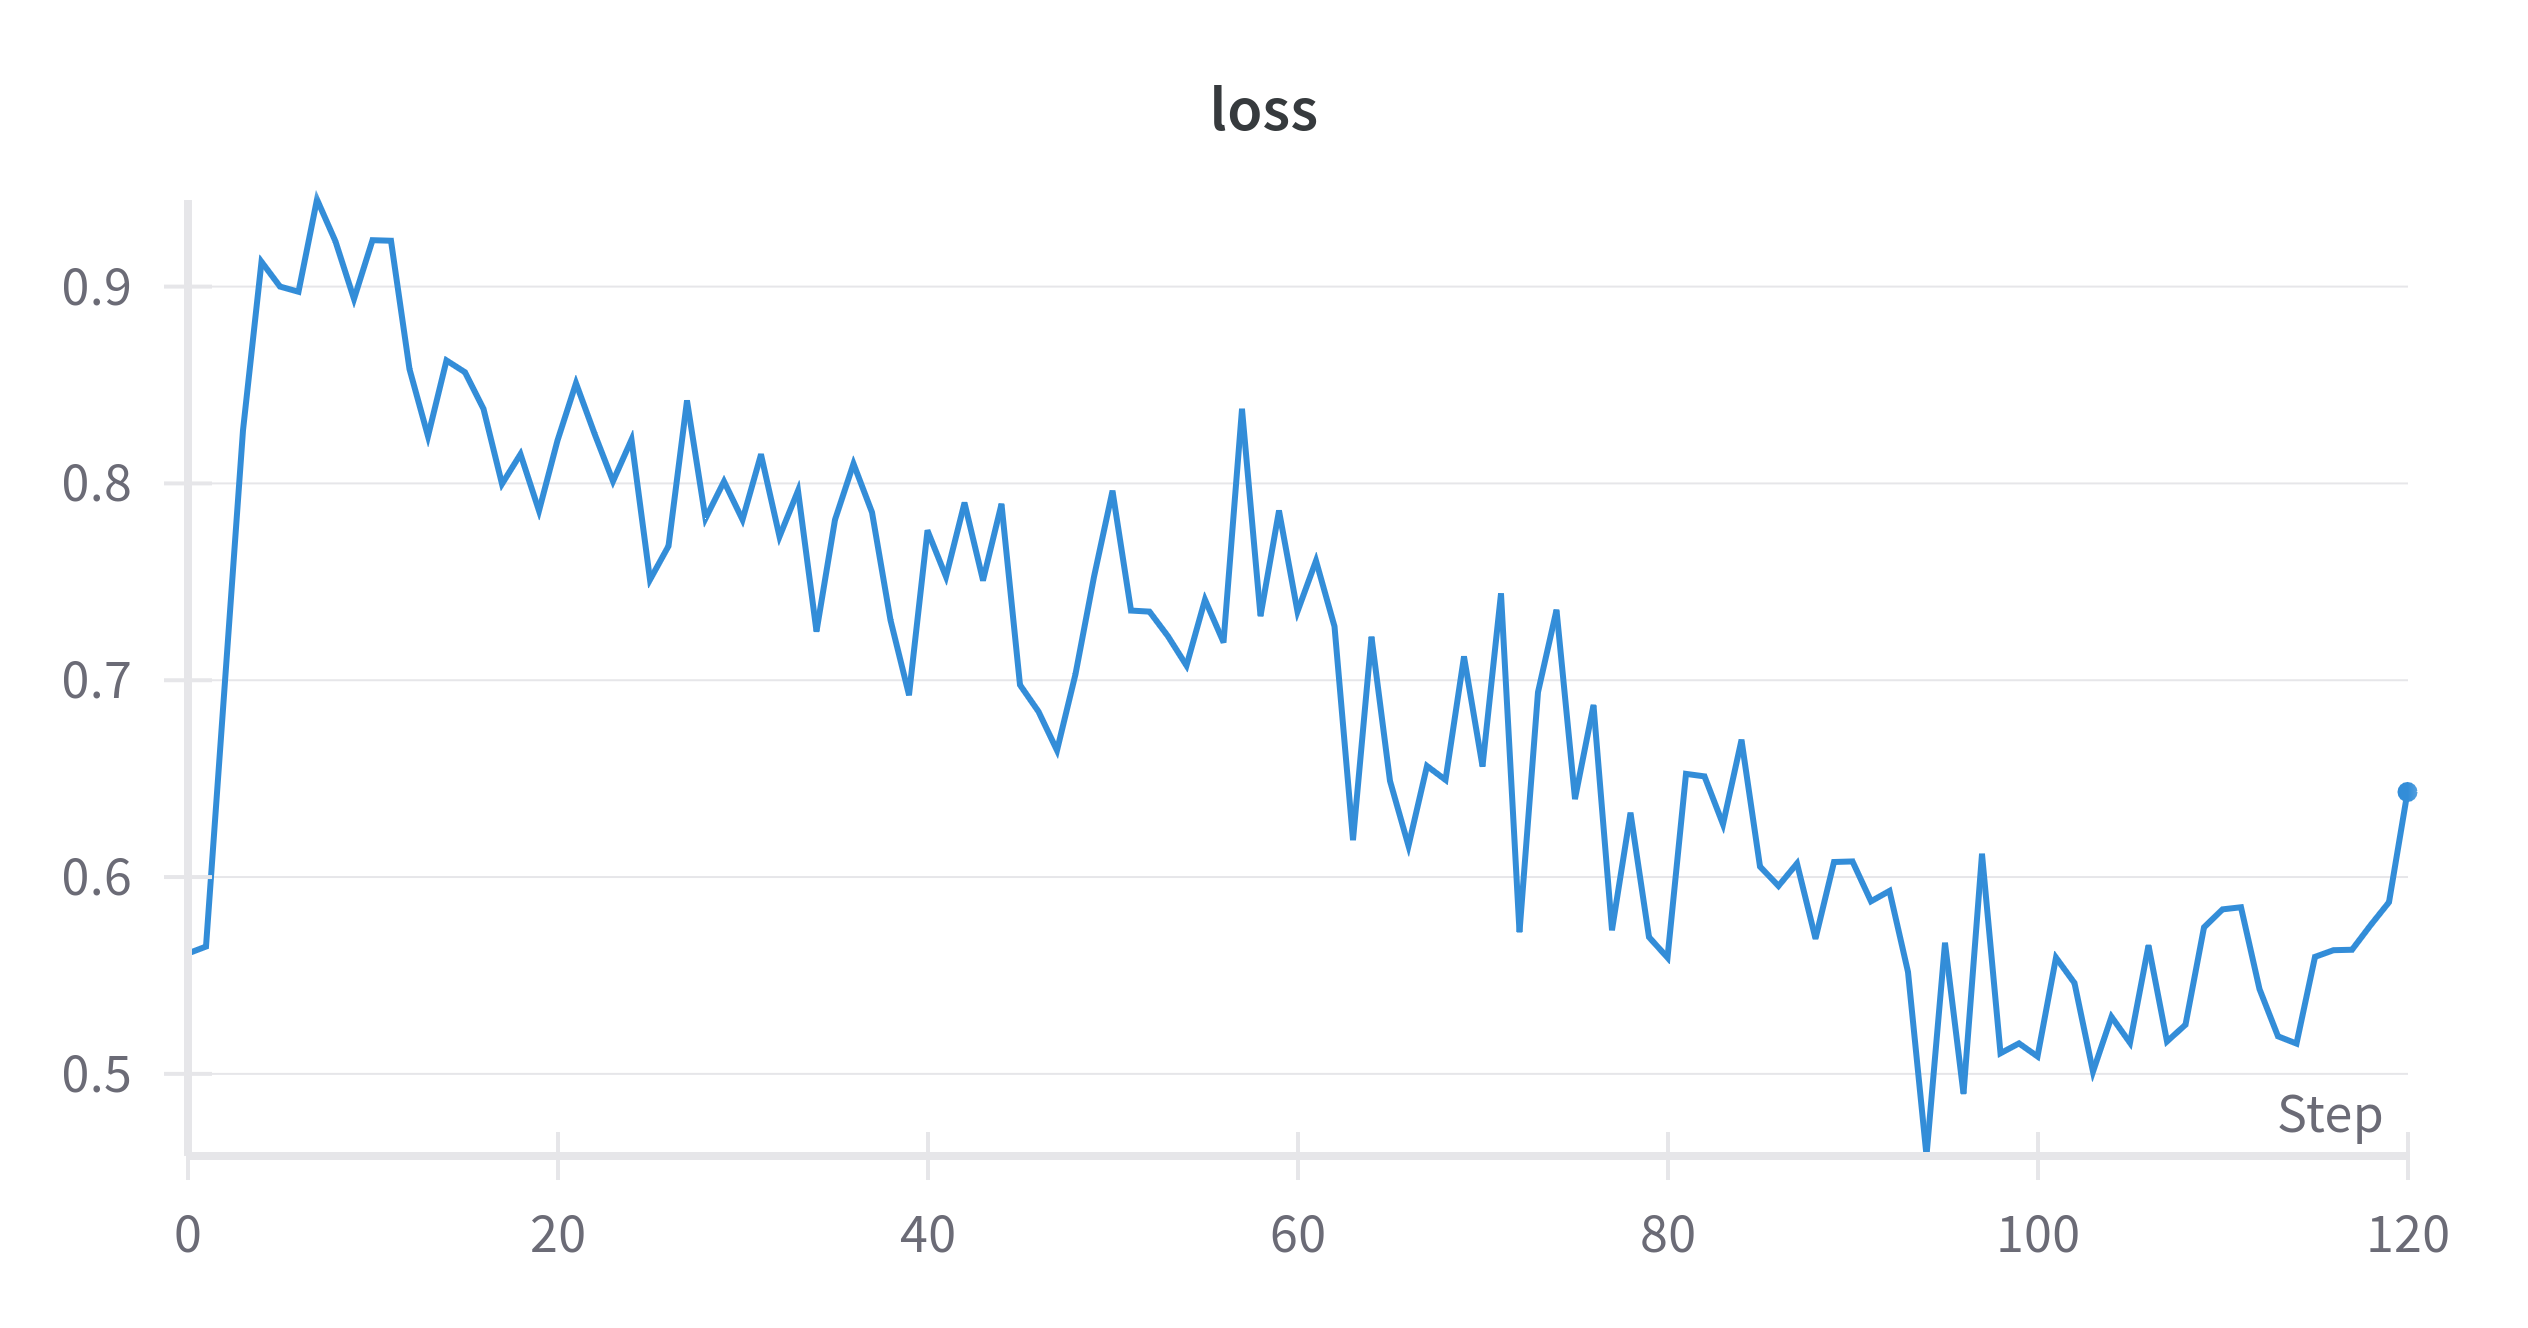
\includegraphics[width=\linewidth]{results/RAINBOW-loss.png}
    \caption{
        Loss curve for Rainbow Agent
    }
    \Description{Loss curve for Rainbow Agent}
    \label{fig:rainbowloss}
\end{figure*}


  \begin{figure*}[h]
    \centering
    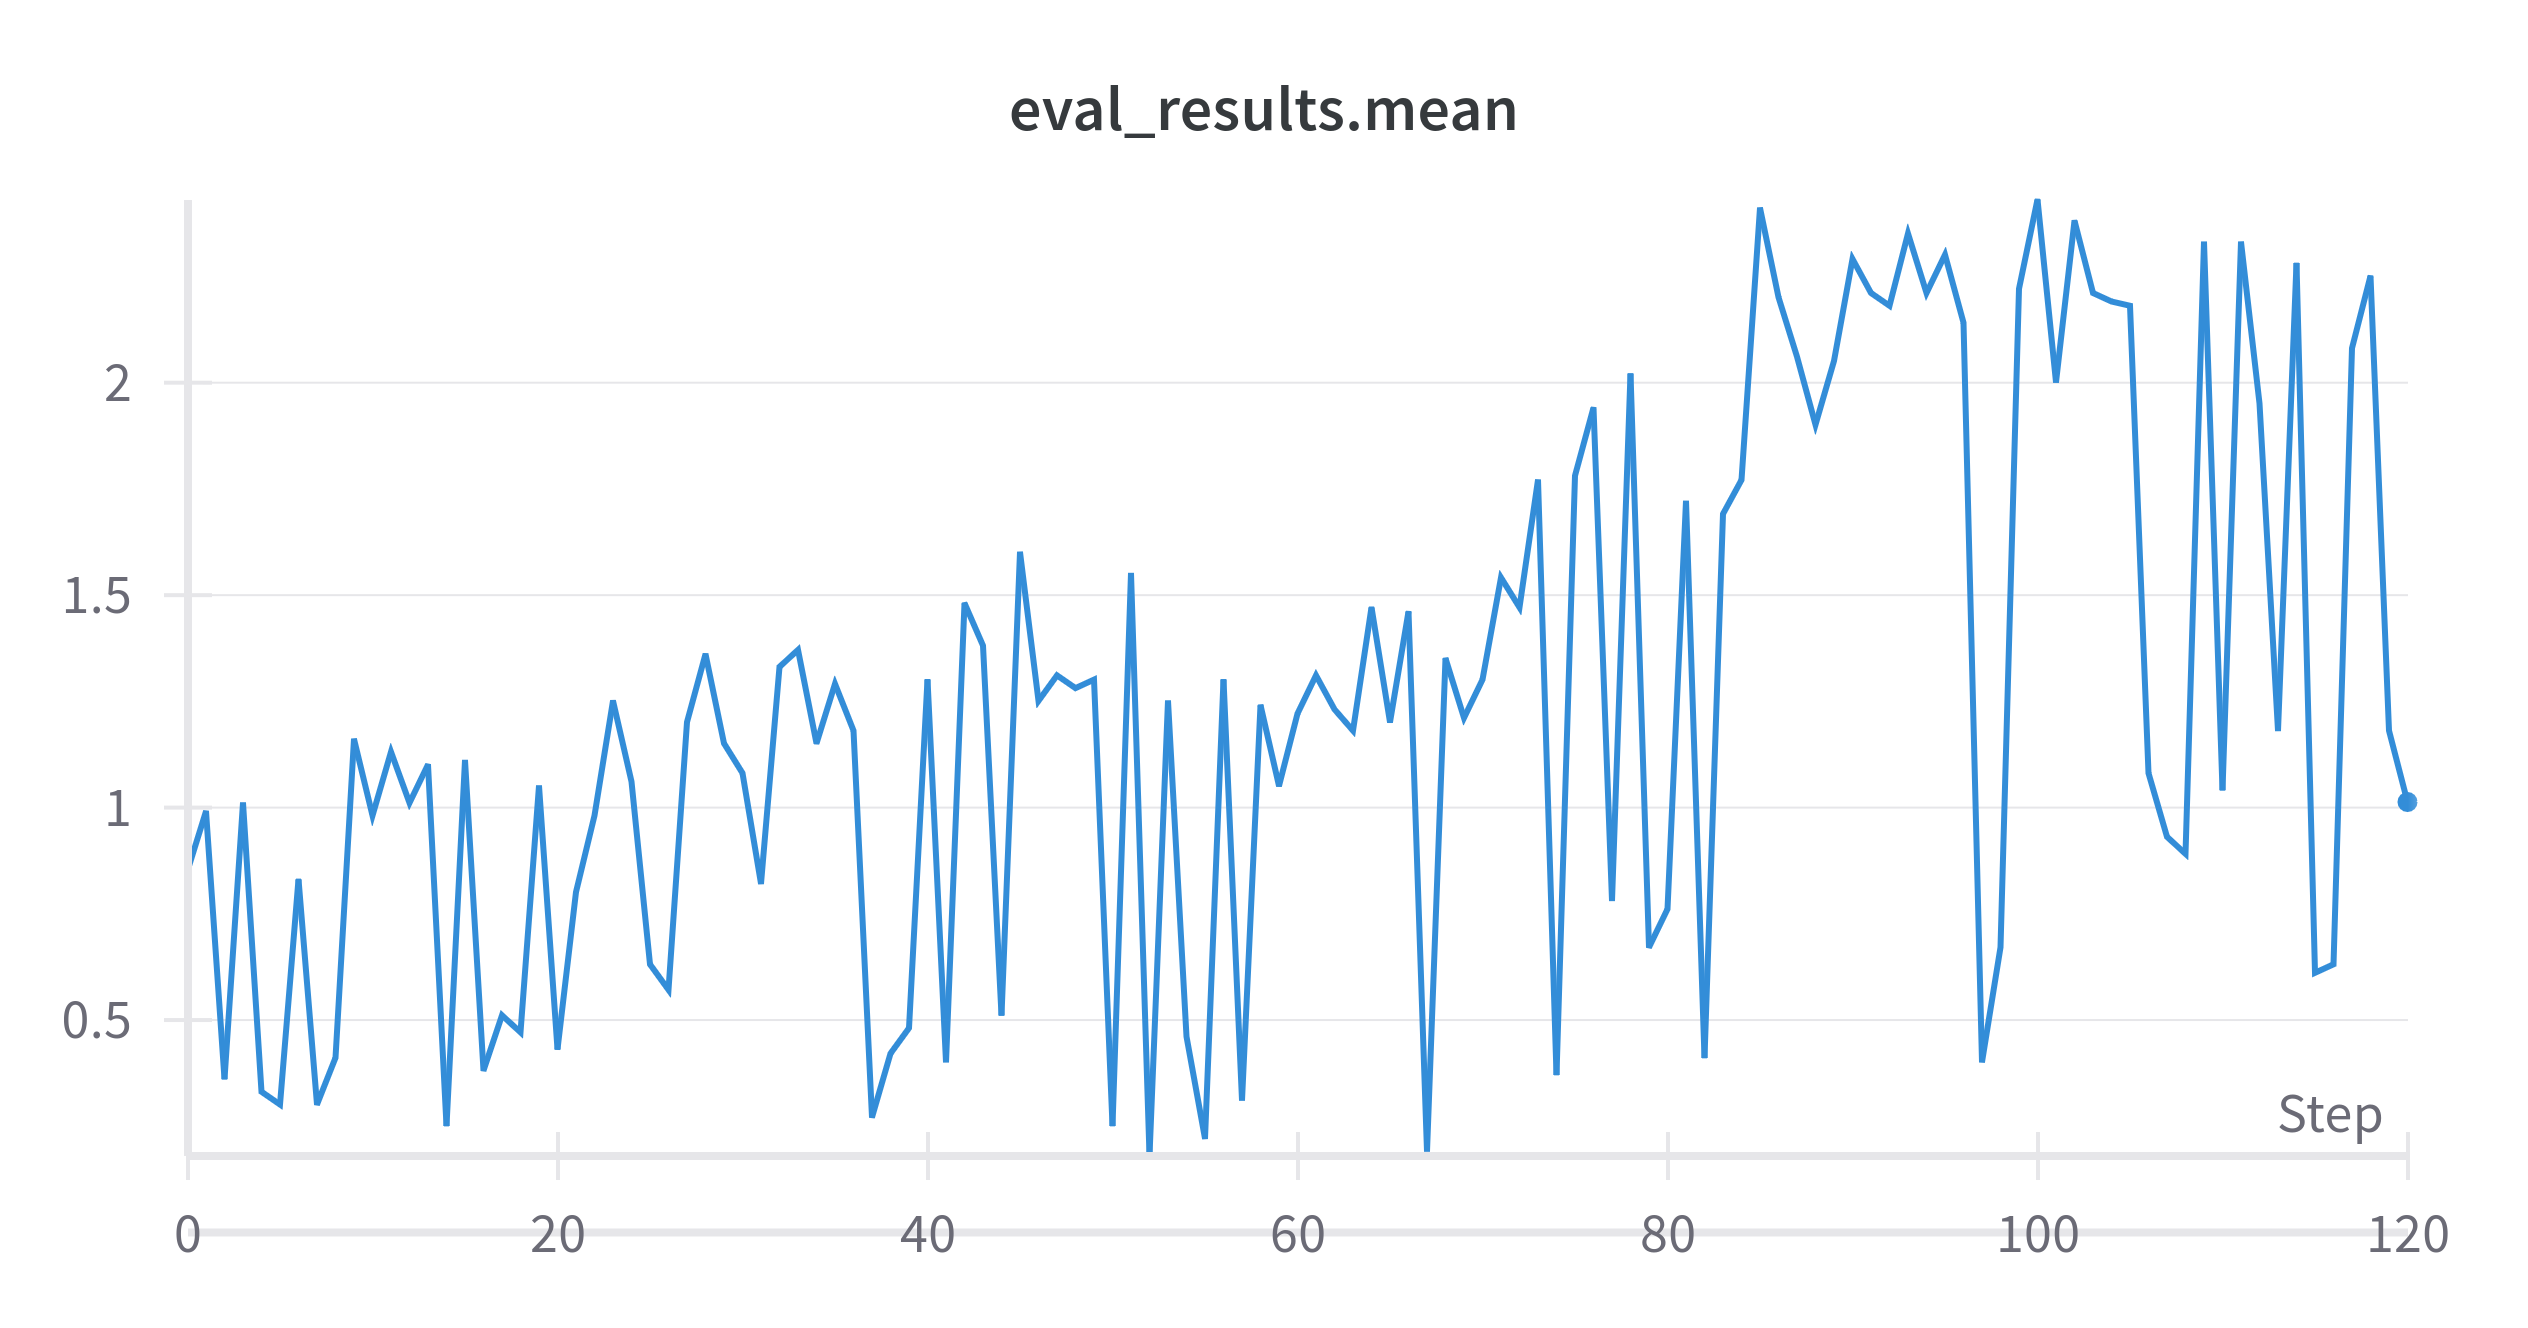
\includegraphics[width=\linewidth]{results/RAINBOW-3-mean.png}
    \caption{
      Training curve for Rainbow-3 Agent
    }
    \Description{Training curve for Rainbow-3 Agent}
    \label{fig:rainbow3}
  \end{figure*}
  \begin{figure*}[h]
    \centering
    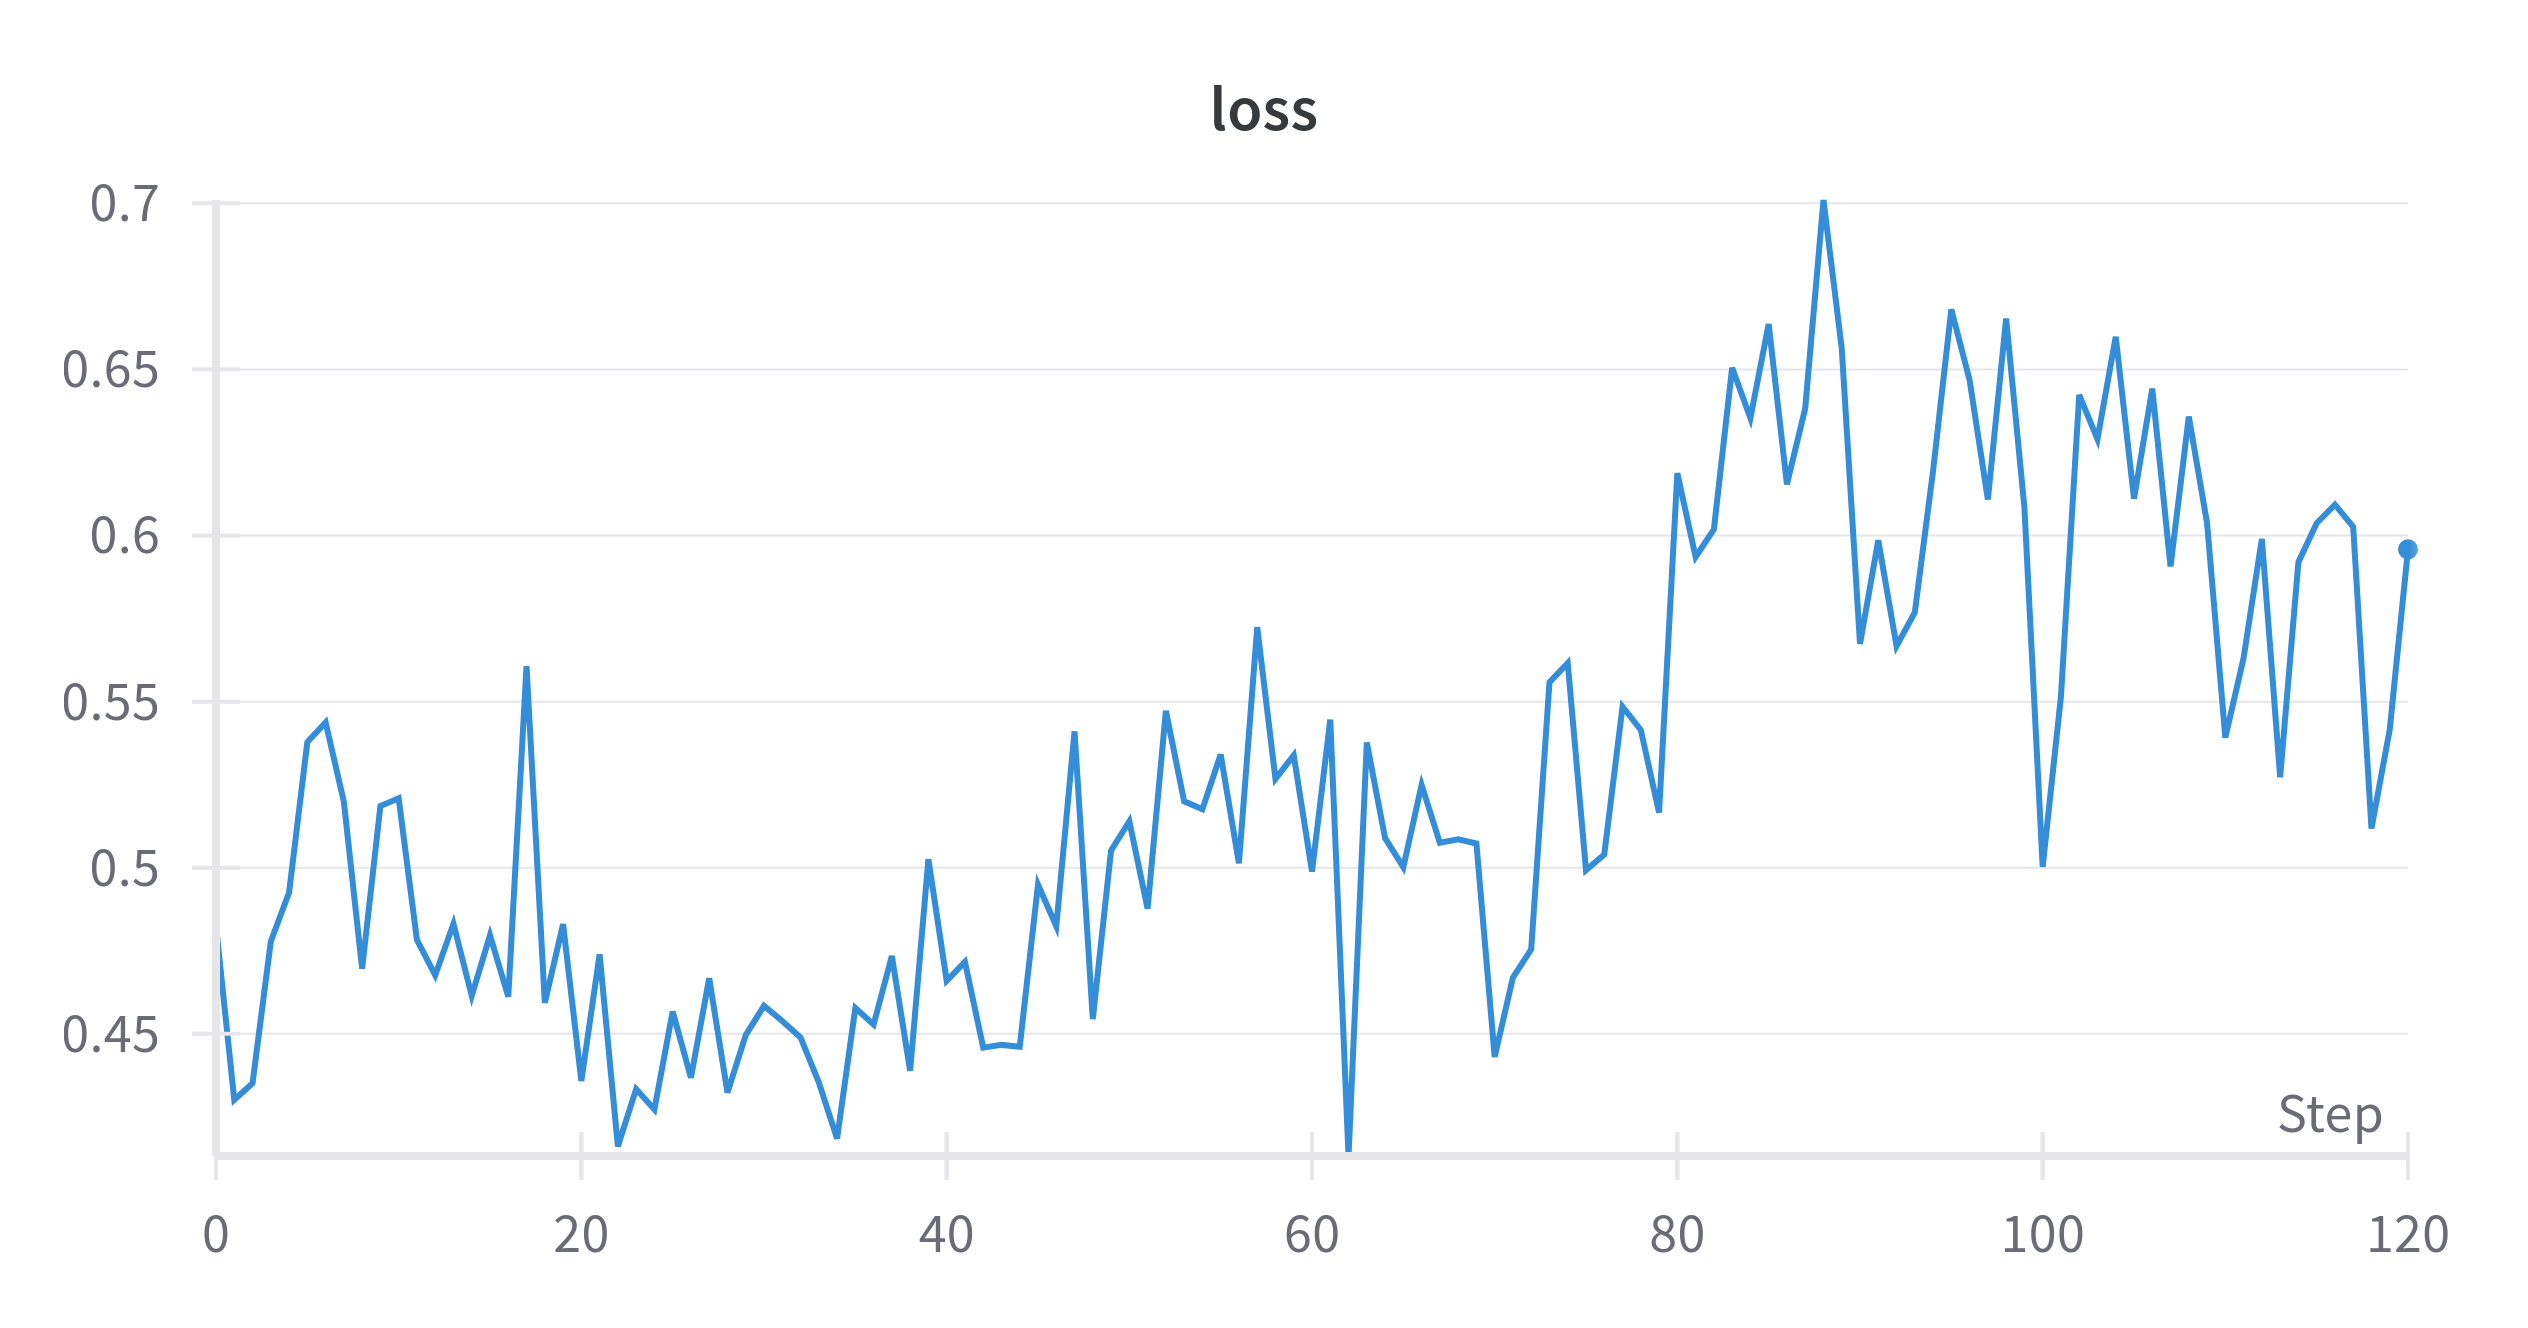
\includegraphics[width=\linewidth]{results/RAINBOW-3-loss.png}
    \caption{
        Loss curve for Rainbow-3 Agent
    }
    \Description{Loss curve for Rainbow-3 Agent}
    \label{fig:rainbow3loss}
\end{figure*}


\begin{figure*}[h]
  \centering
  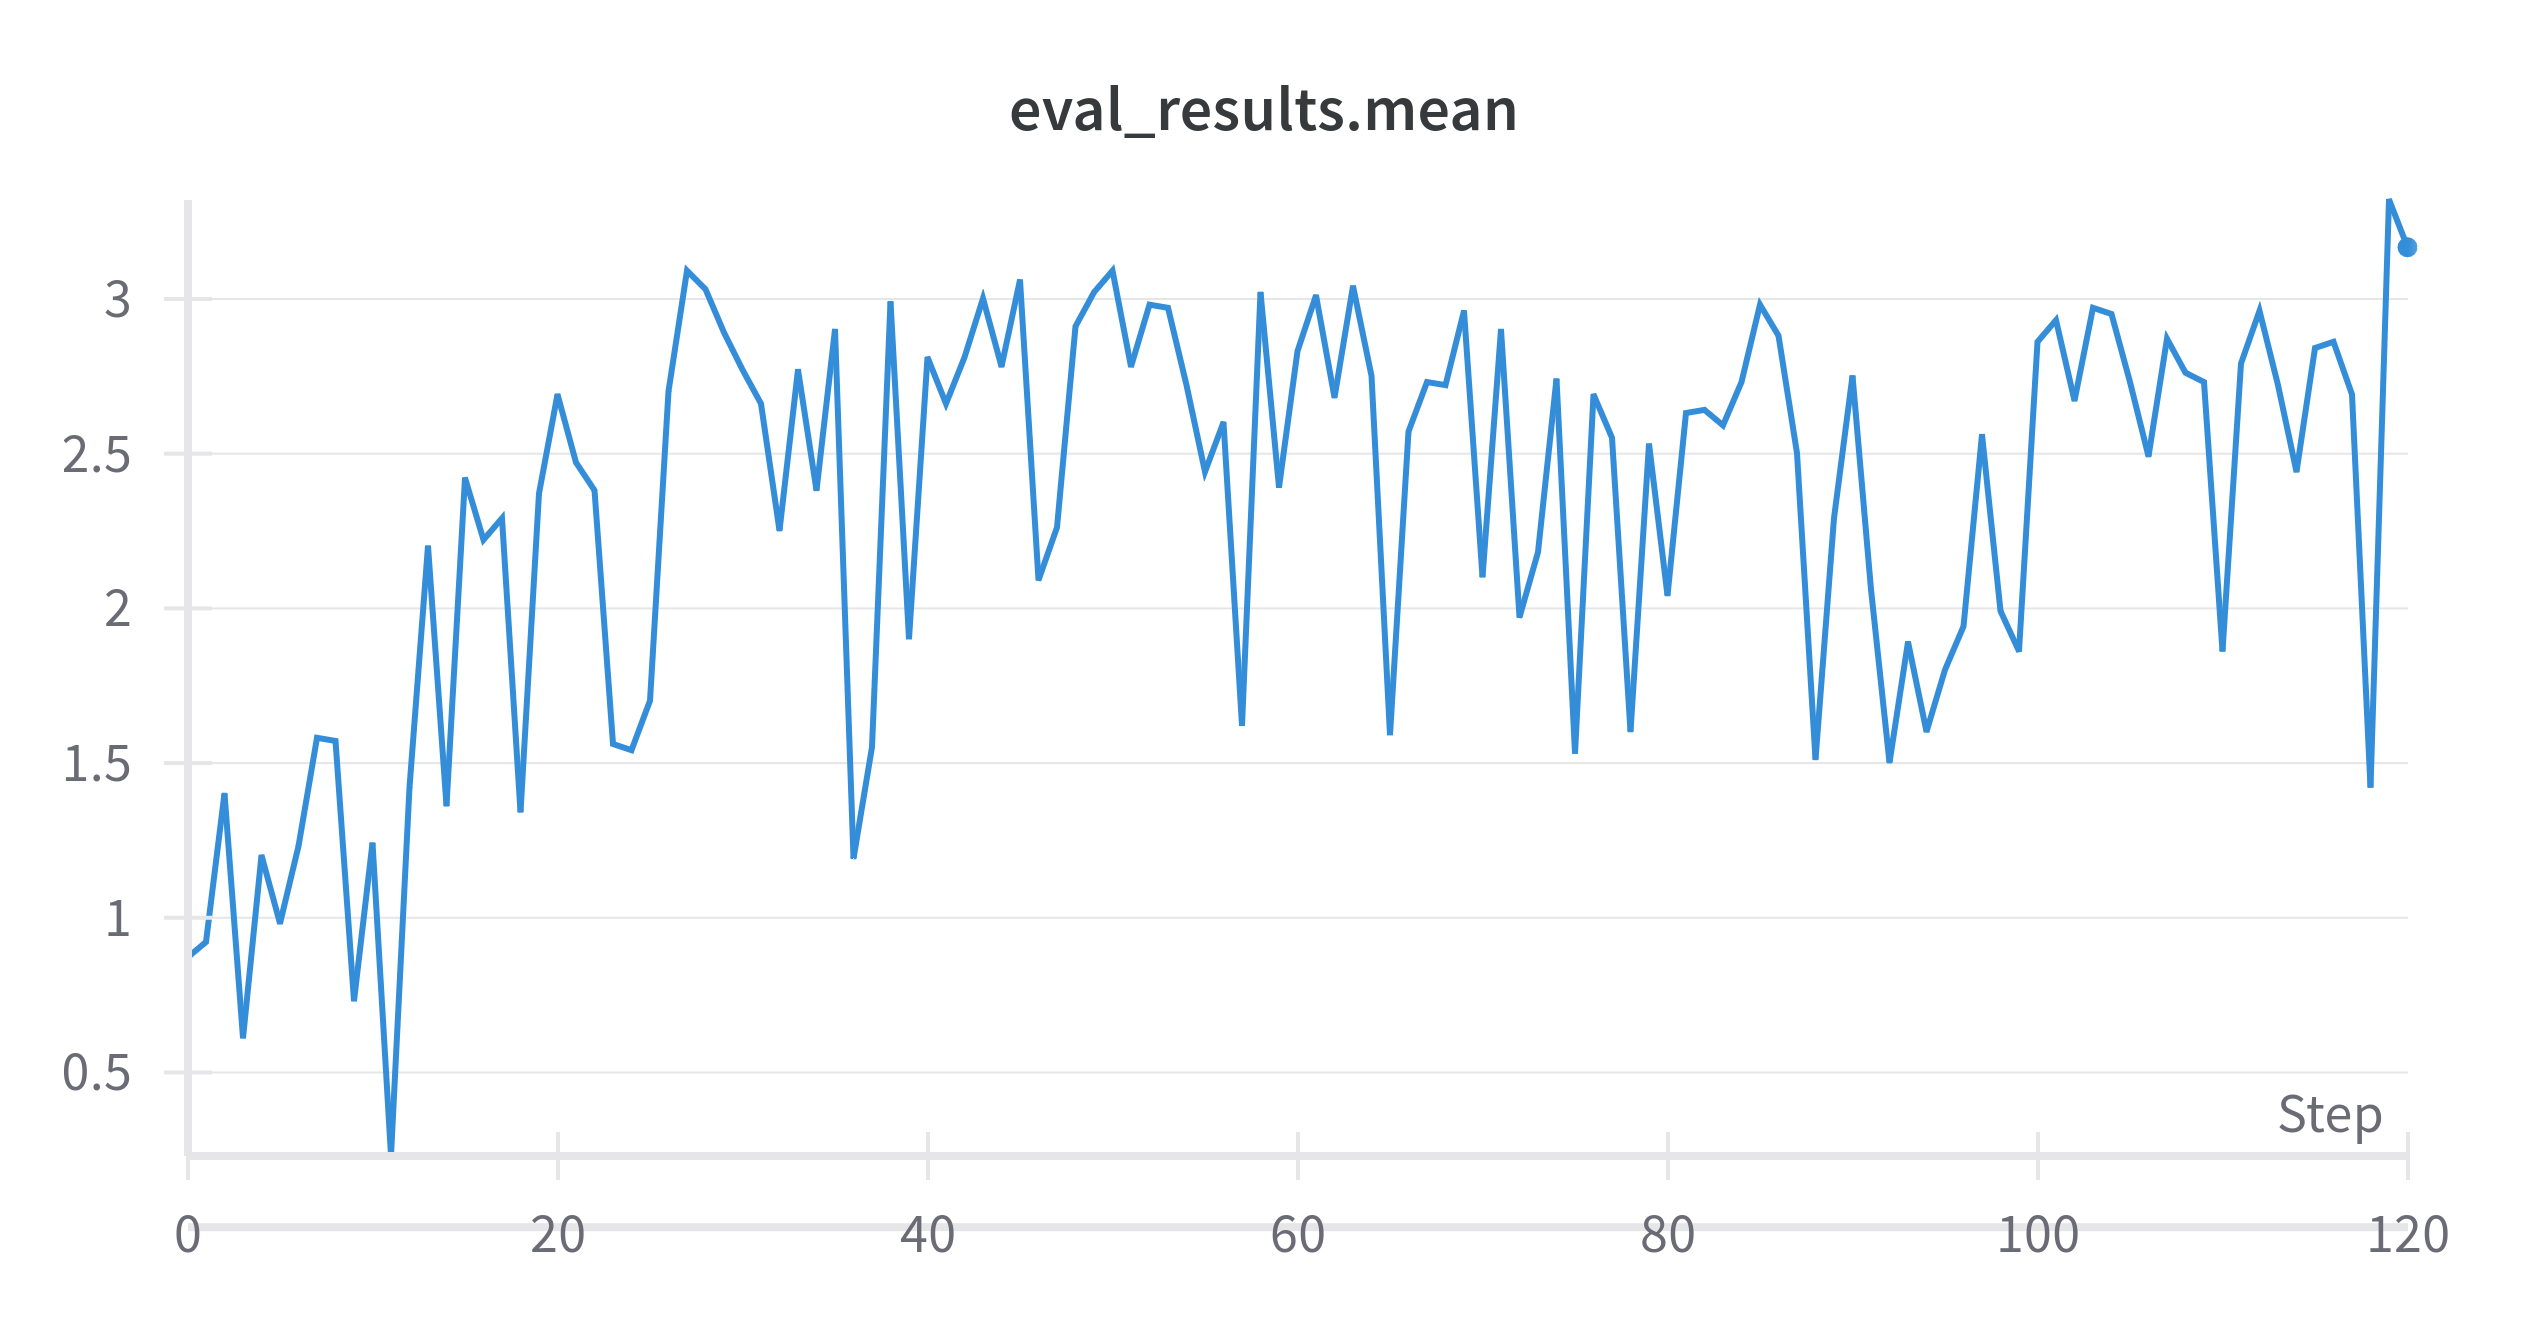
\includegraphics[width=\linewidth]{results/RAINBOW-5-mean.png}
  \caption{
    Training curve for Rainbow-5 Agent
  }
  \Description{Training curve for Rainbow-5 Agent}
  \label{fig:rainbow5}
\end{figure*}

\begin{figure*}[h]
  \centering
  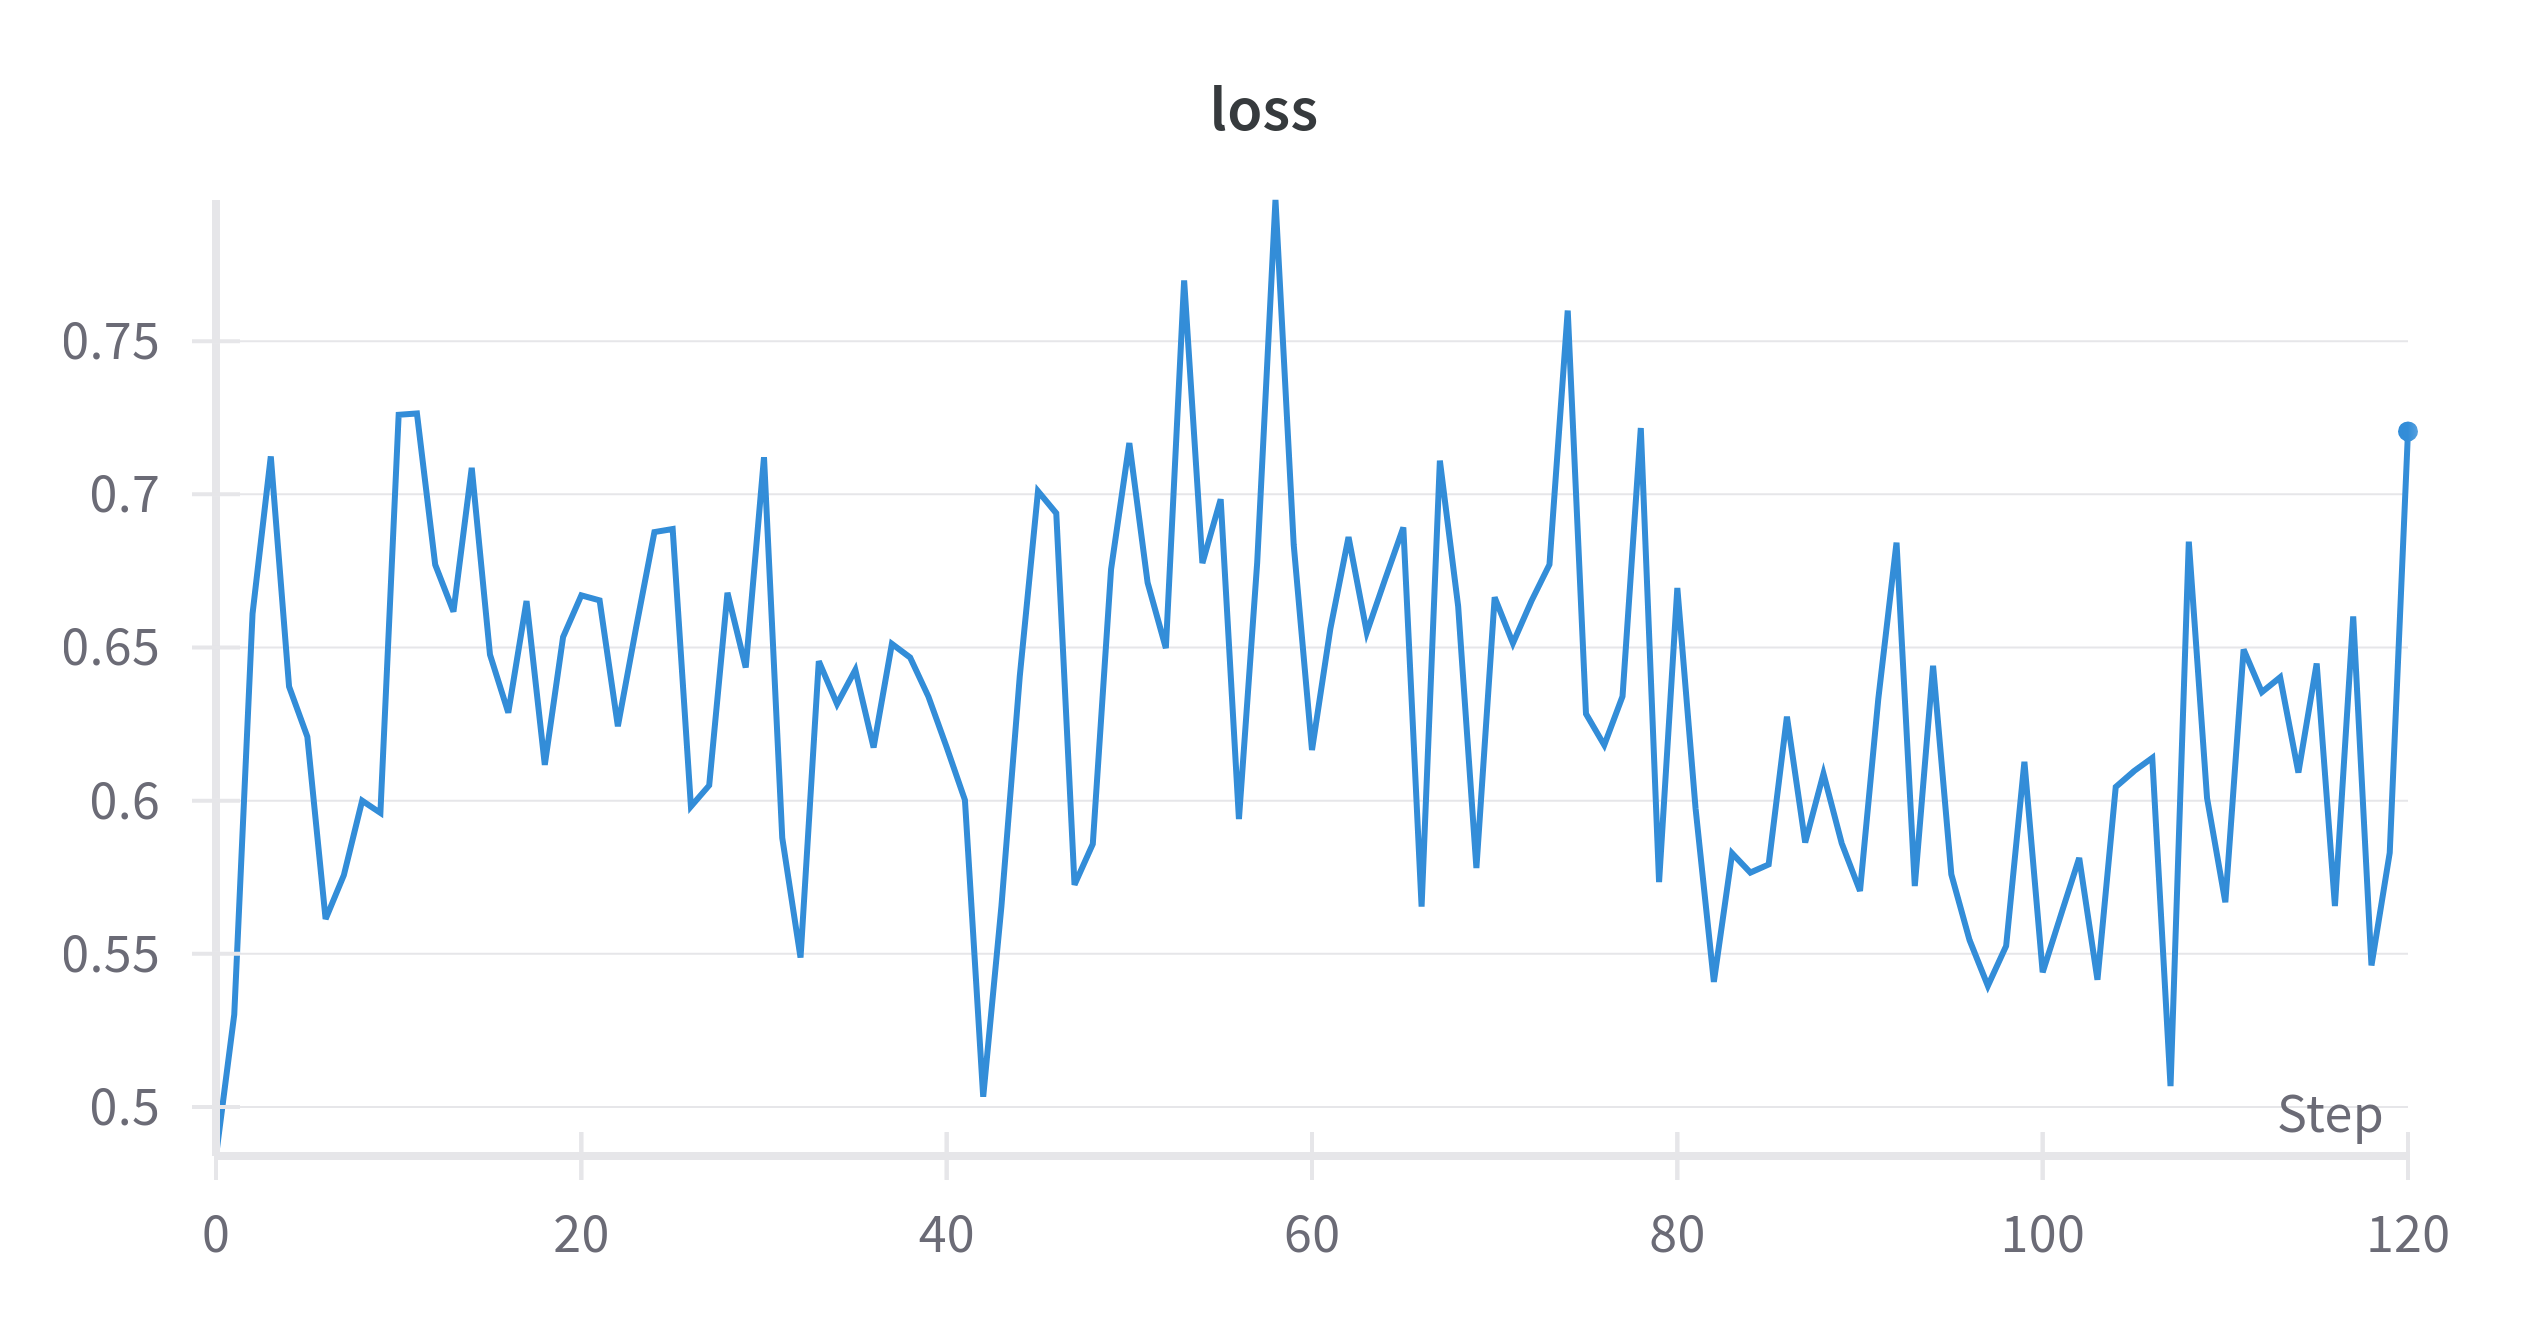
\includegraphics[width=\linewidth]{results/RAINBOW-5-loss.png}
  \caption{
      Loss curve for Rainbow-5 Agent
  }
  \Description{Loss curve for Rainbow-5 Agent}
  \label{fig:rainbow5loss}
\end{figure*}


  \begin{figure*}[h]
    \centering
    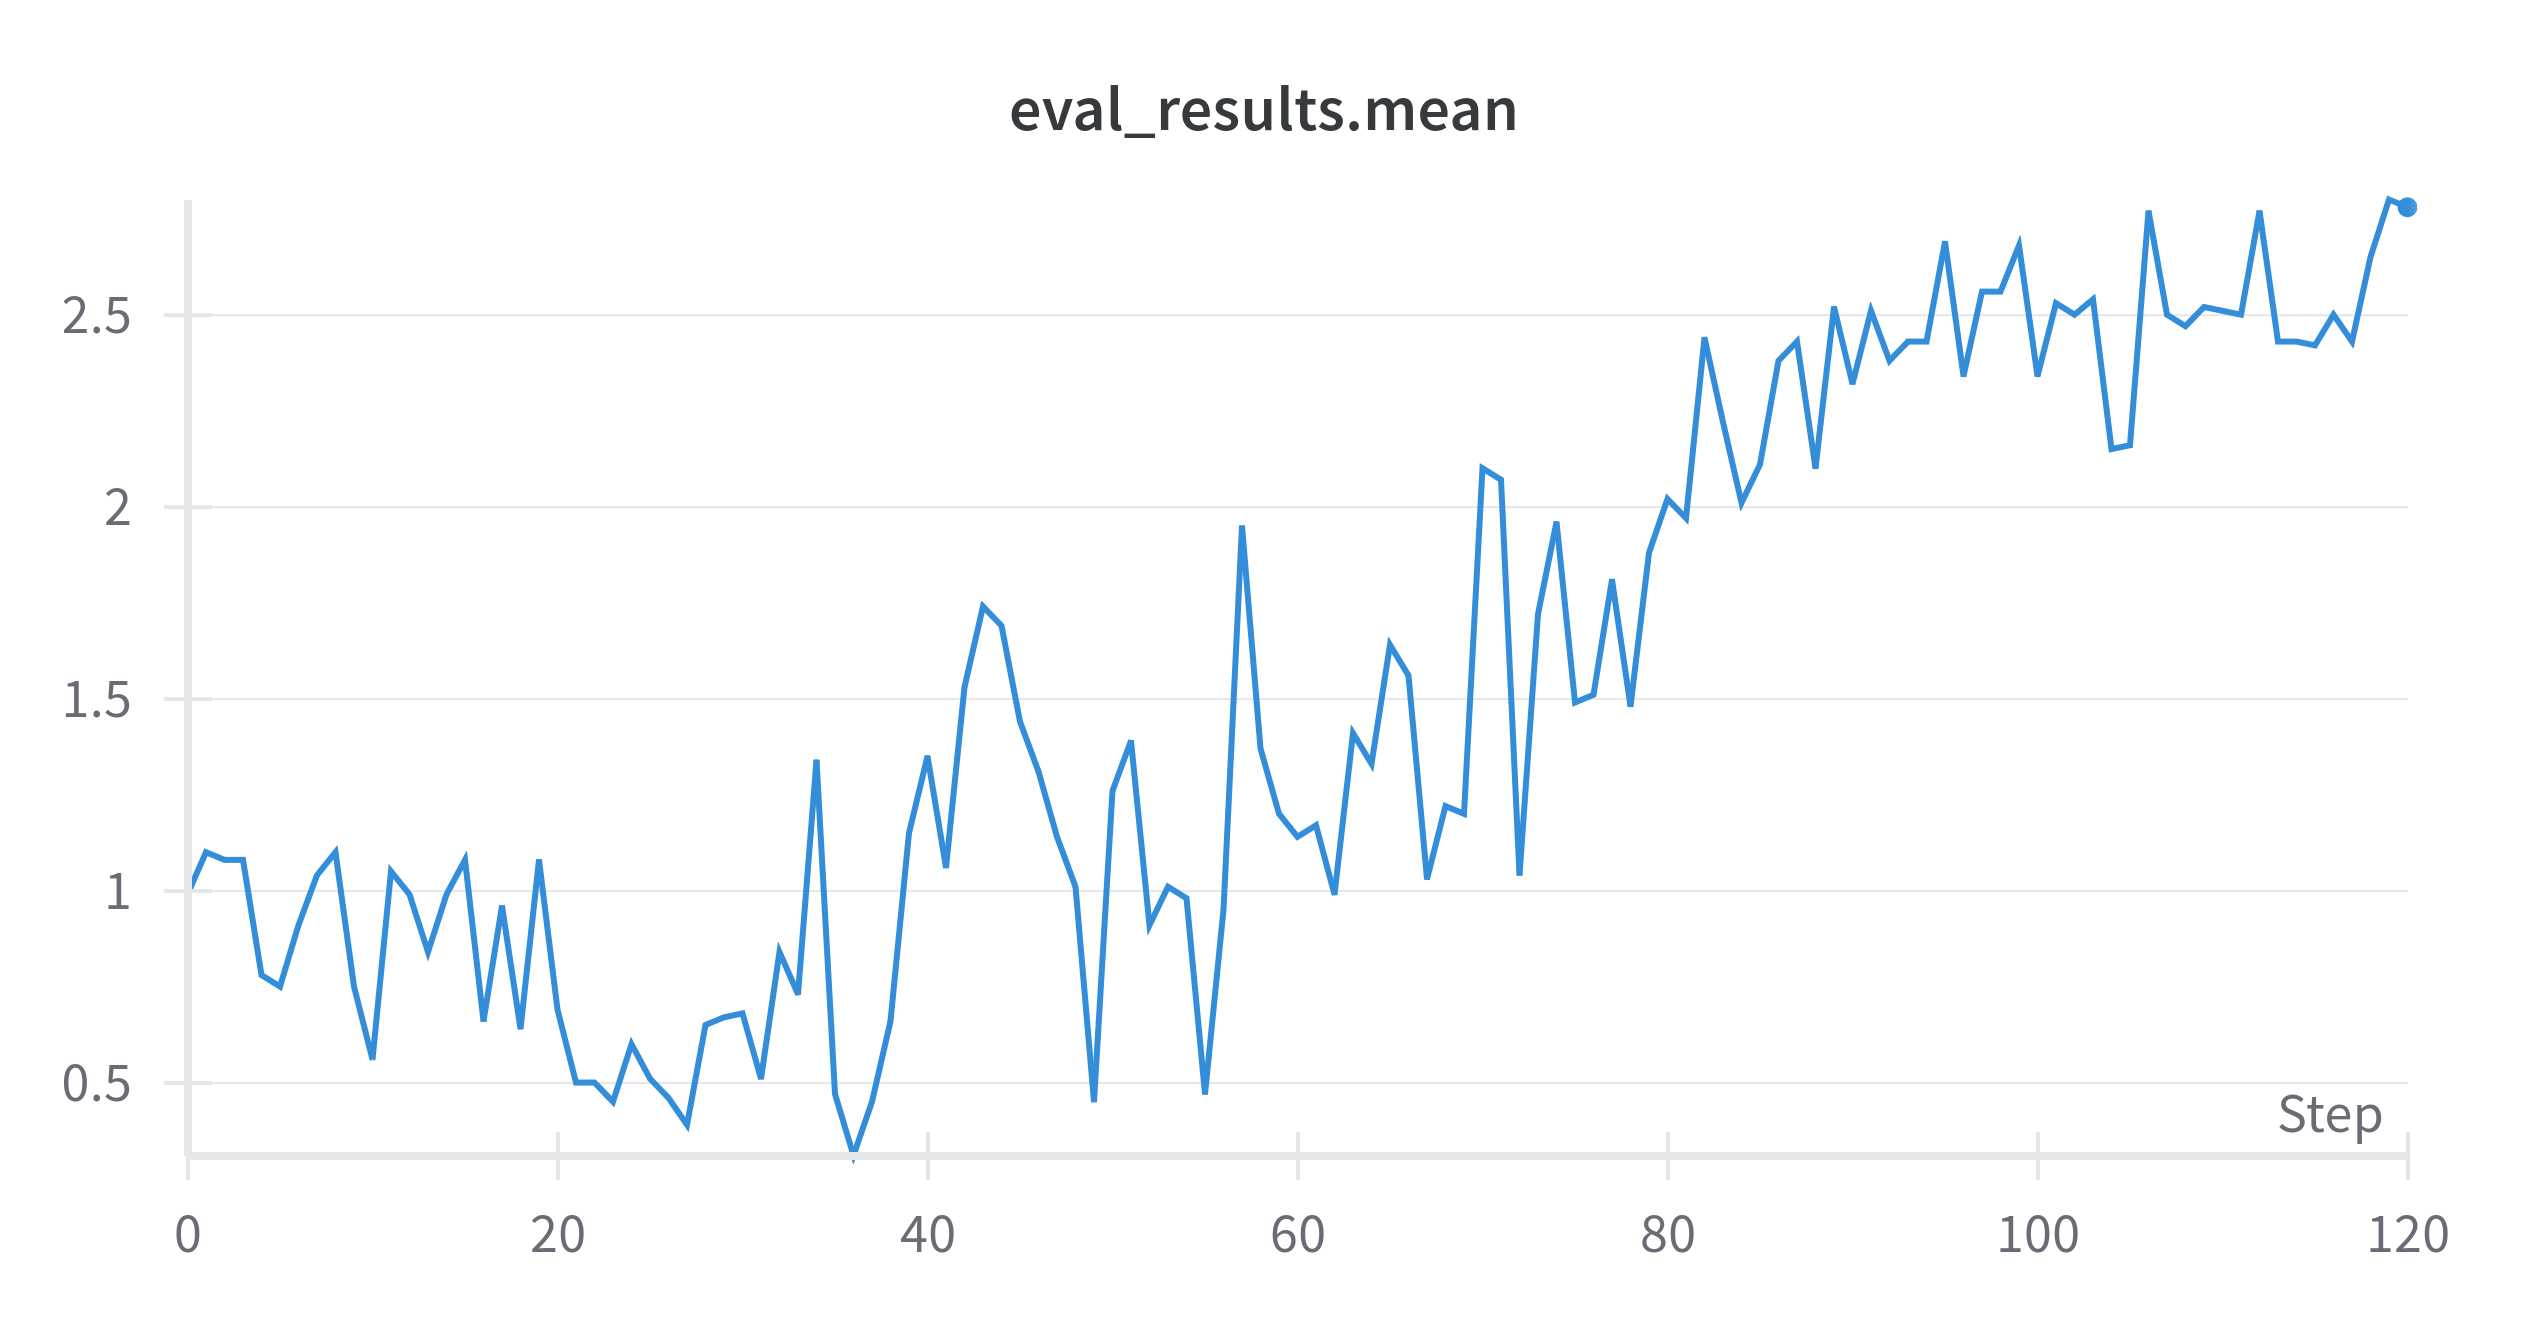
\includegraphics[width=\linewidth]{results/Distributed-mean.png}
    \caption{
      Training curve for Distributed Agent
    }
    \Description{Training curve for Distributed Agent}
    \label{fig:distributed}
  \end{figure*}


\begin{figure*}[h]
  \centering
  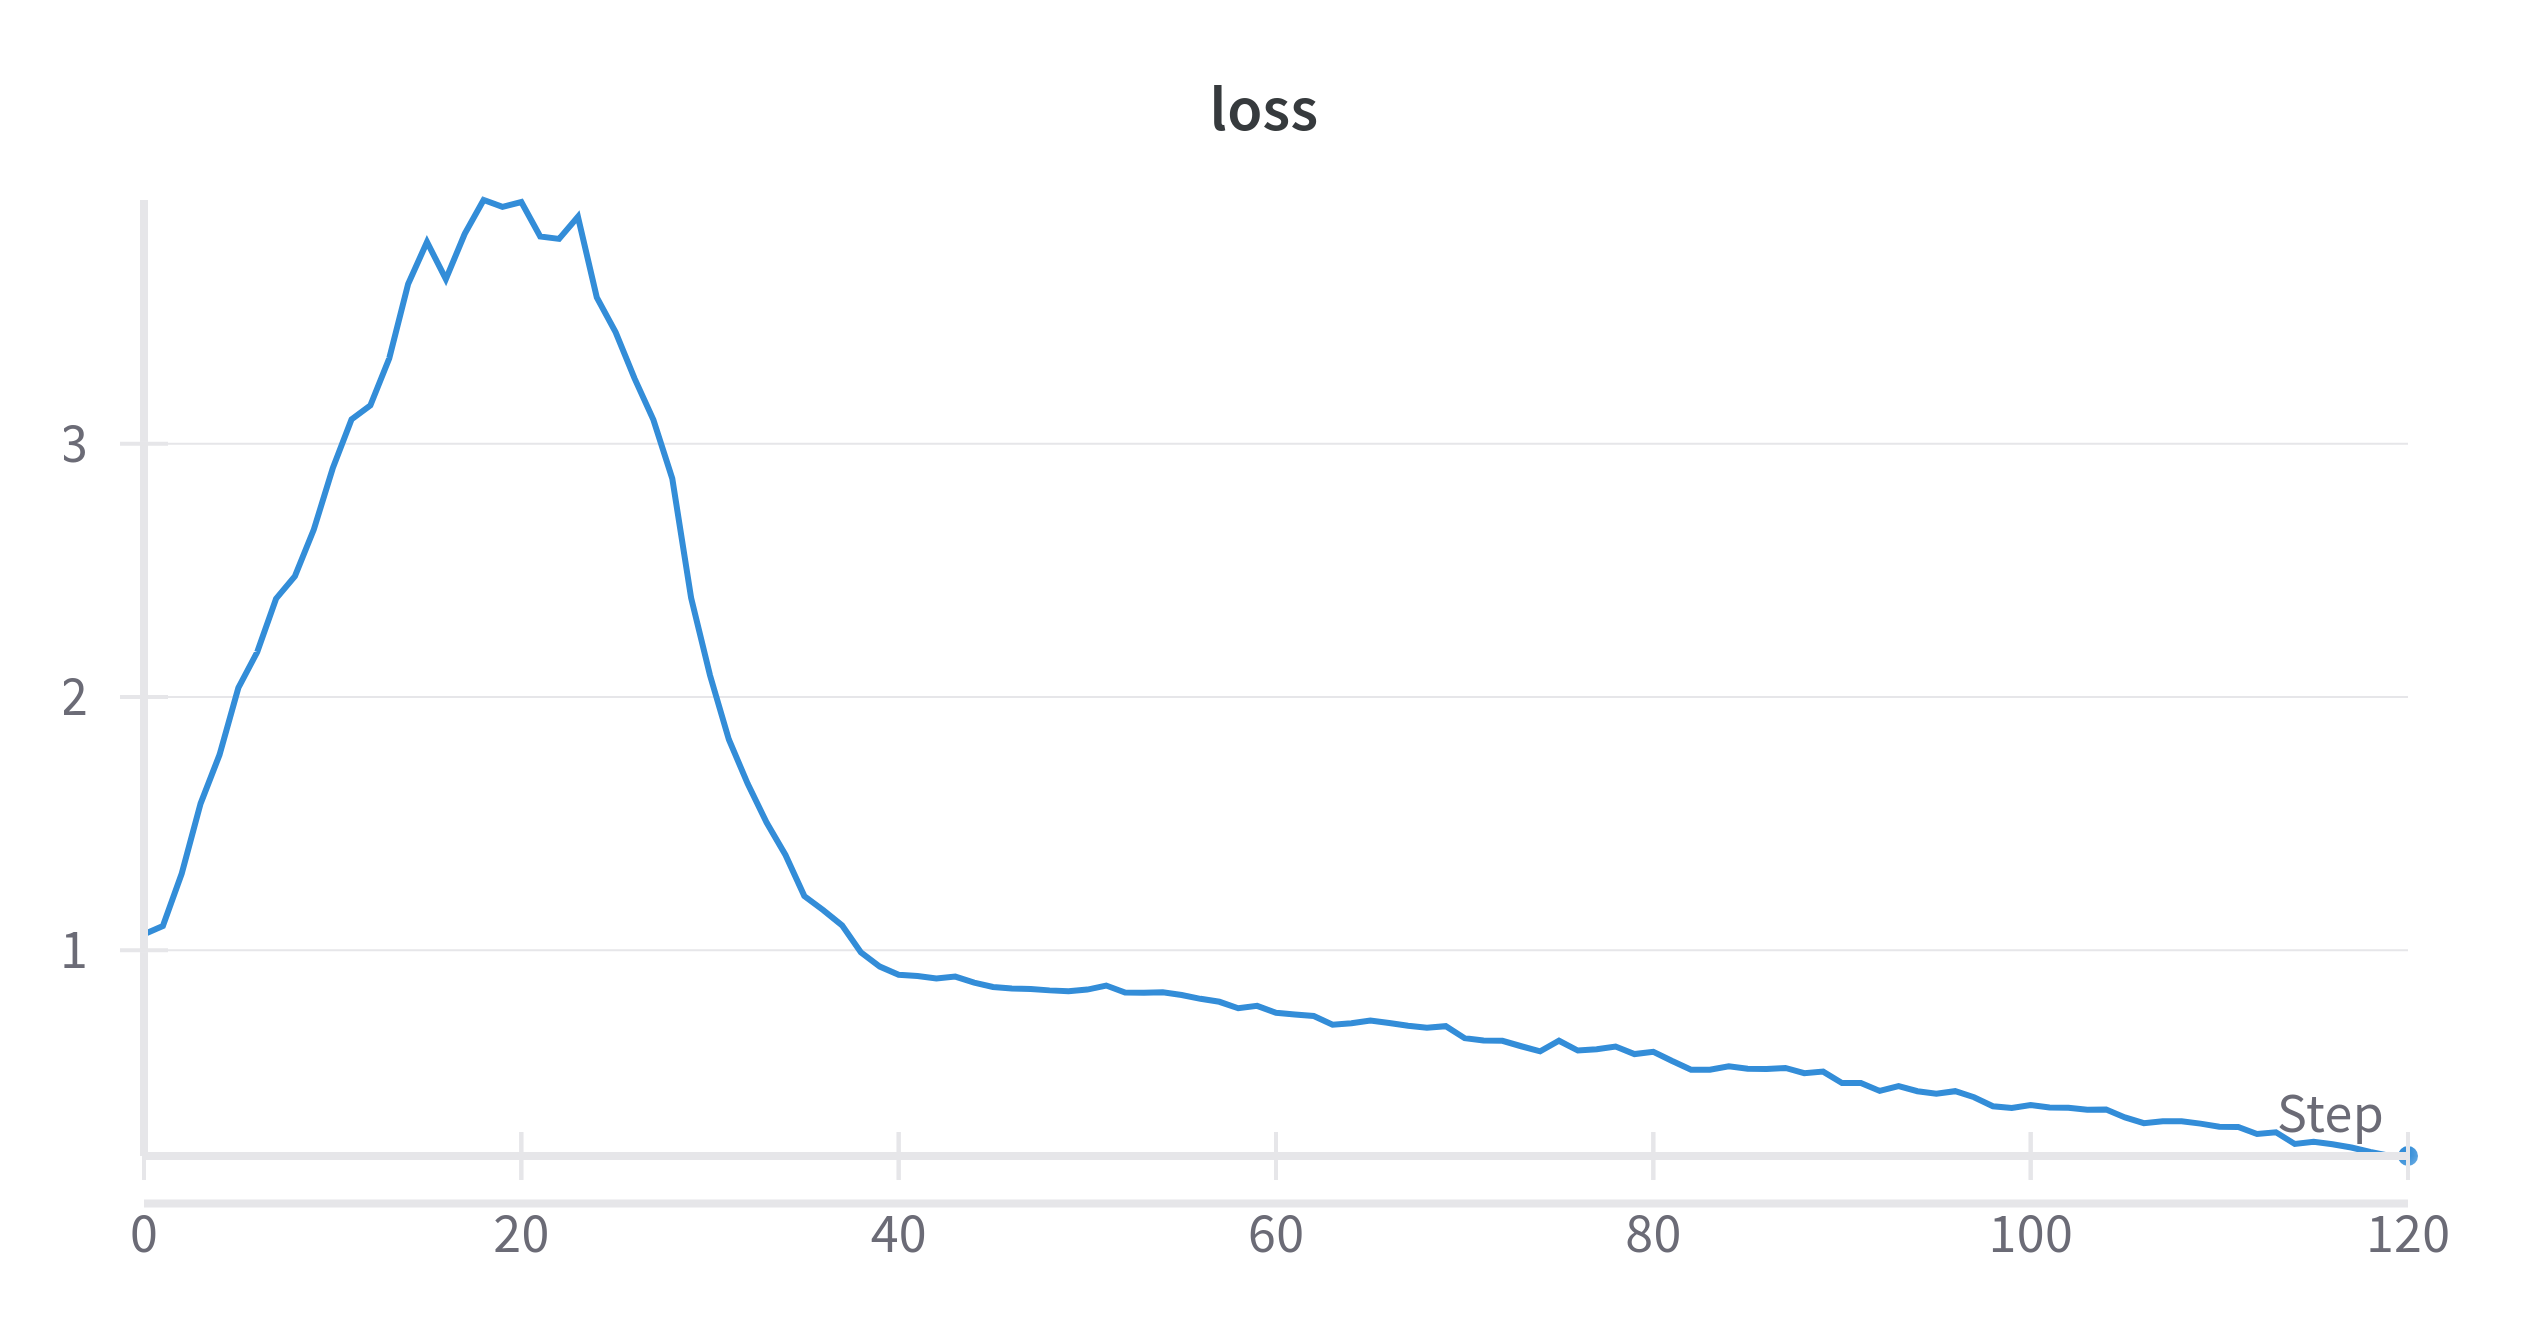
\includegraphics[width=\linewidth]{results/Distributed-loss.png}
  \caption{
      Loss curve for Distributed Agent
  }
  \Description{Loss curve for Distributed Agent}
  \label{fig:distributedloss}
\end{figure*}

  
  \begin{figure*}[h]
    \centering
    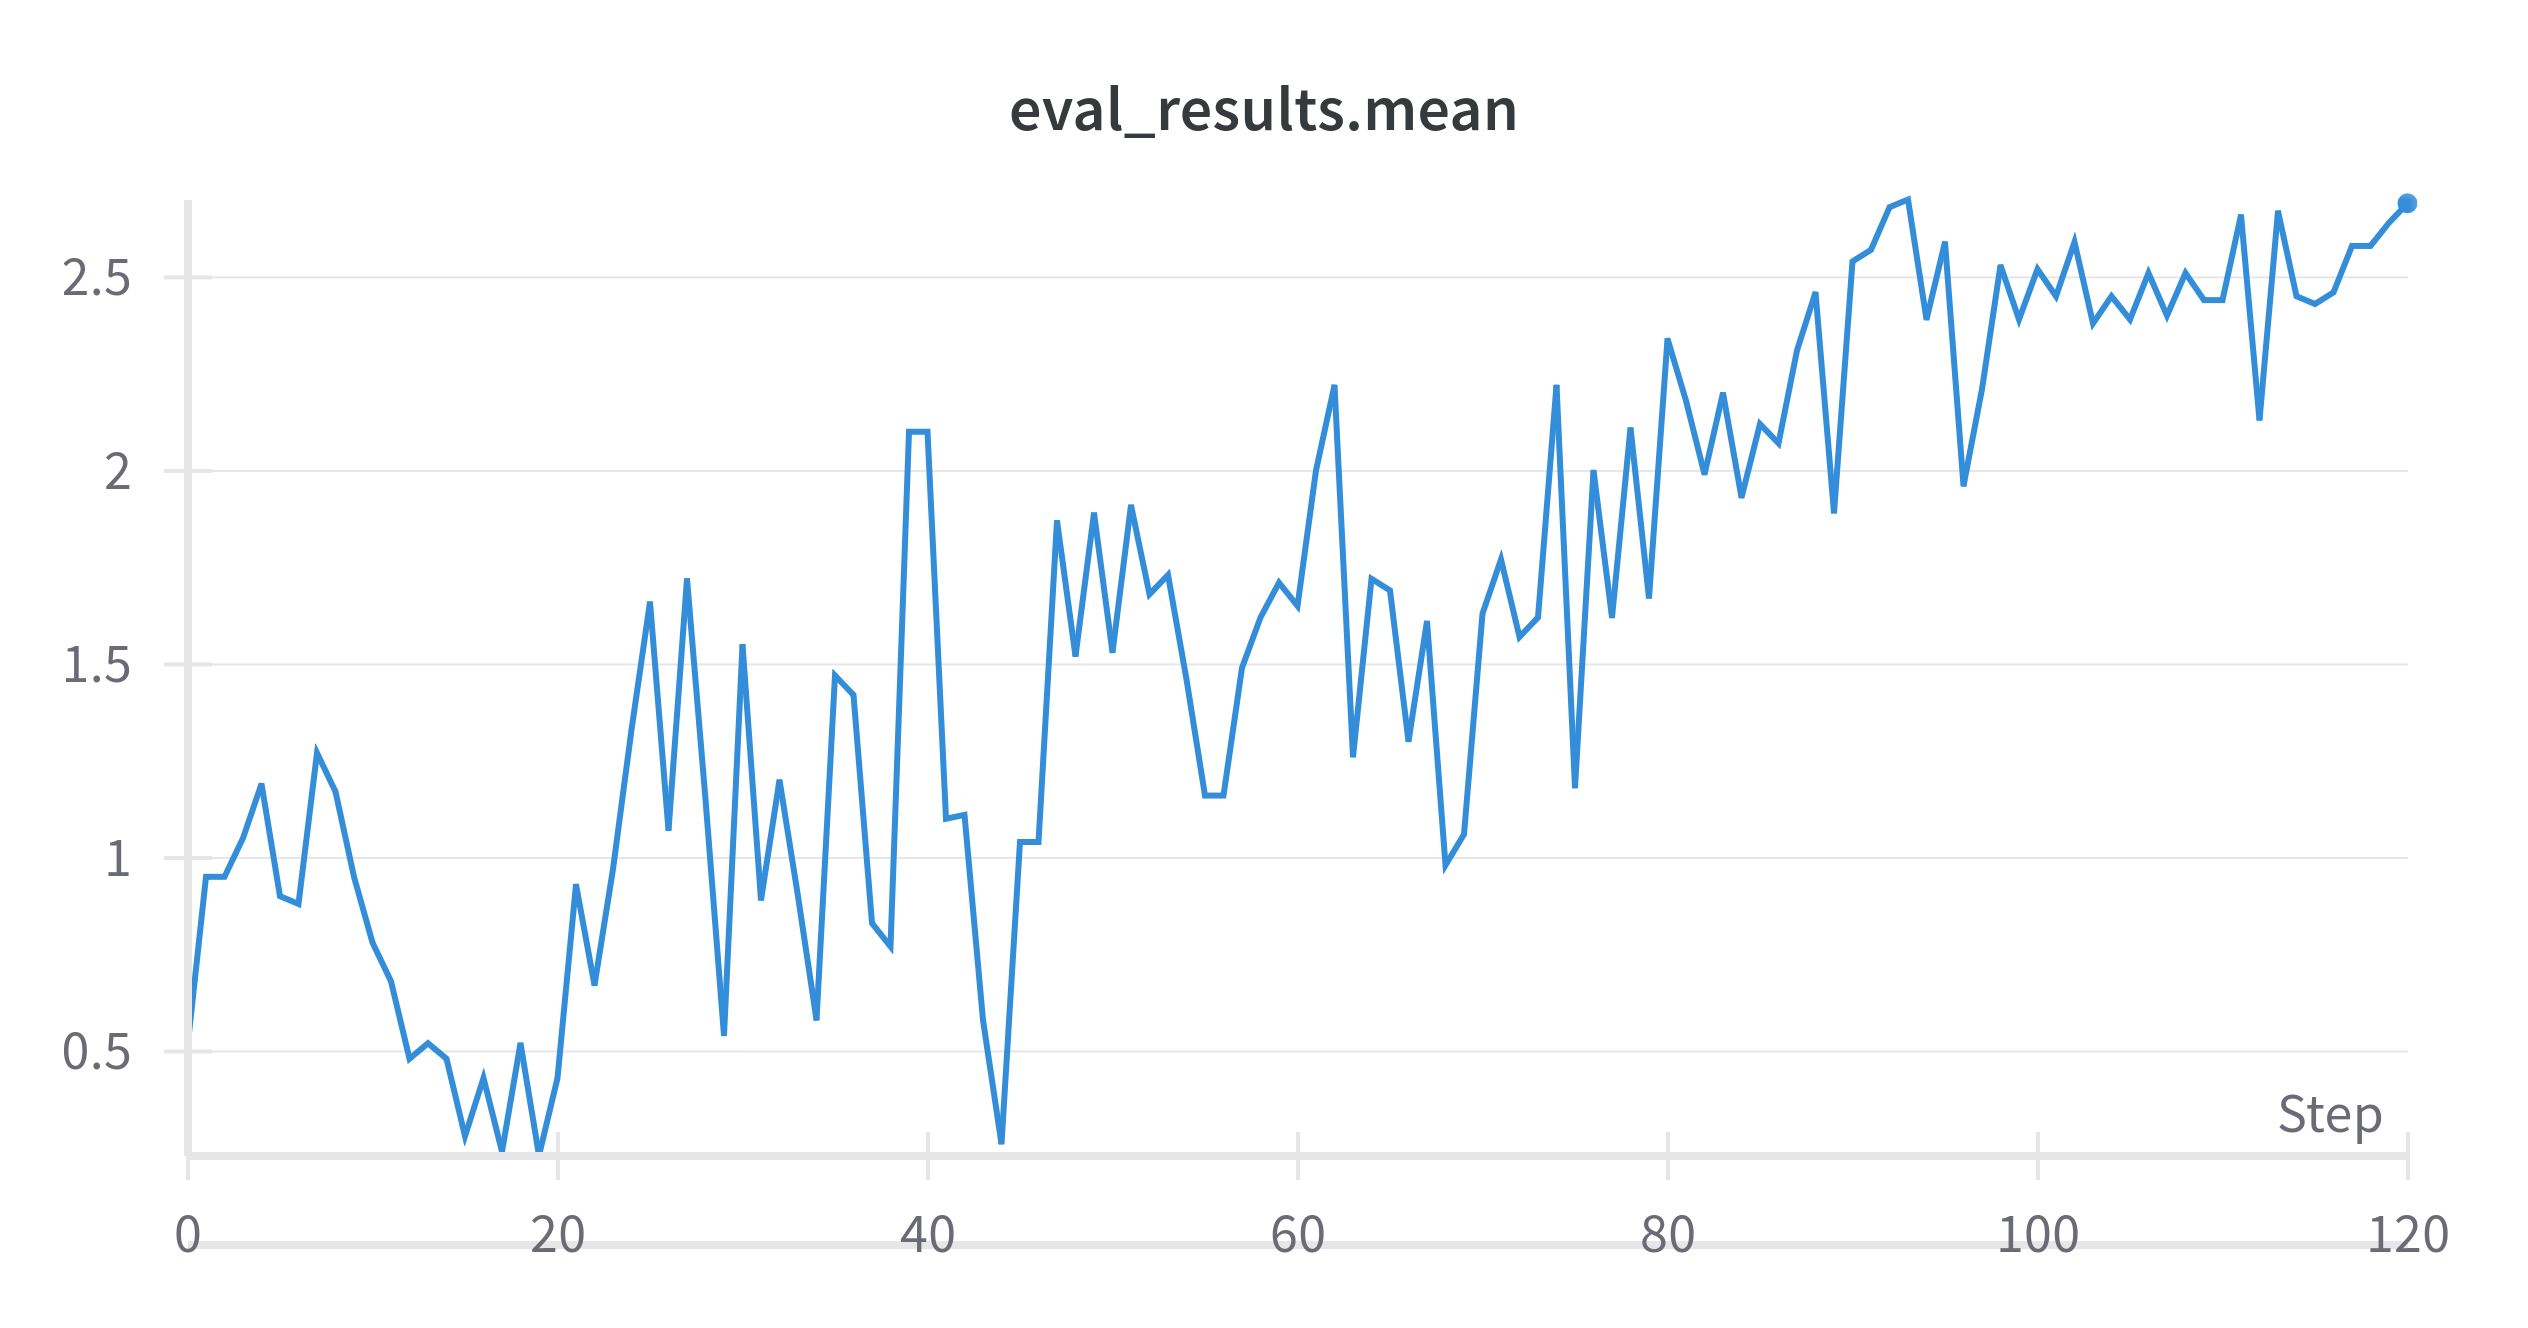
\includegraphics[width=\linewidth]{results/SAD-mean.png}
    \caption{
      Training curve for SAD Agent
    }
    \Description{Training curve for SAD Agent}
    \label{fig:sad}
  \end{figure*}
  
\begin{figure*}[h]
  \centering
  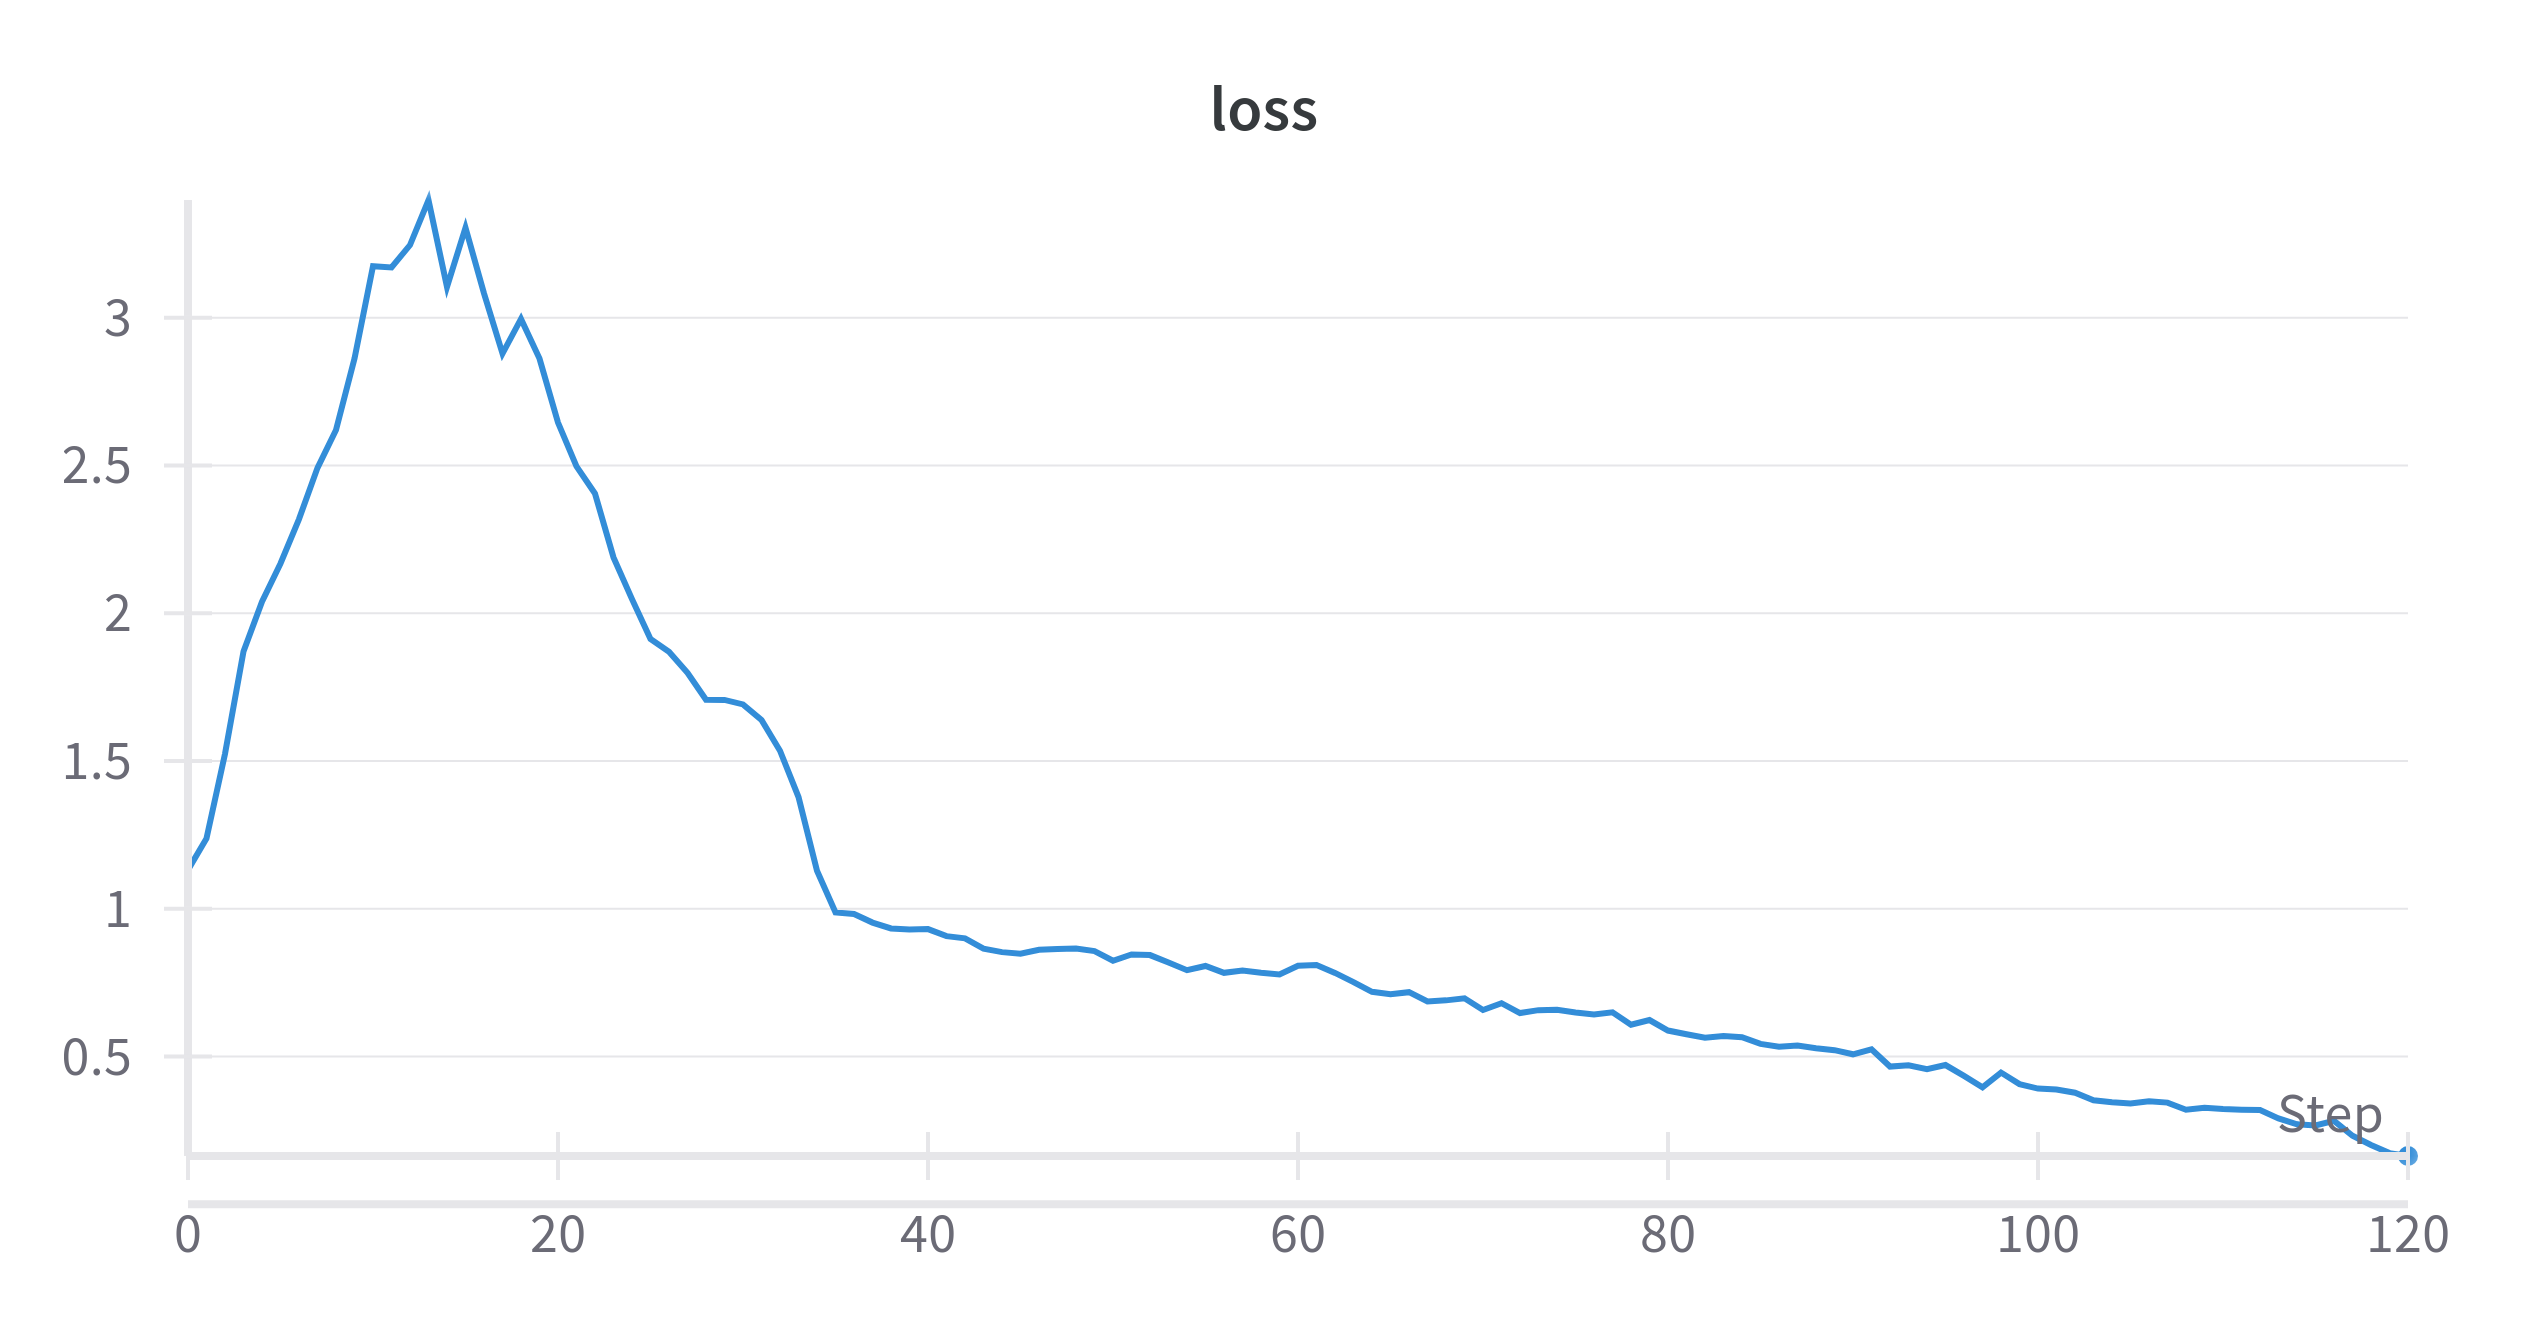
\includegraphics[width=\linewidth]{results/SAD-loss.png}
  \caption{
      Loss curve for SAD Agent
  }
  \Description{Loss curve for SAD Agent}
  \label{fig:sadloss}
\end{figure*}


  \begin{figure*}[h]
    \centering
    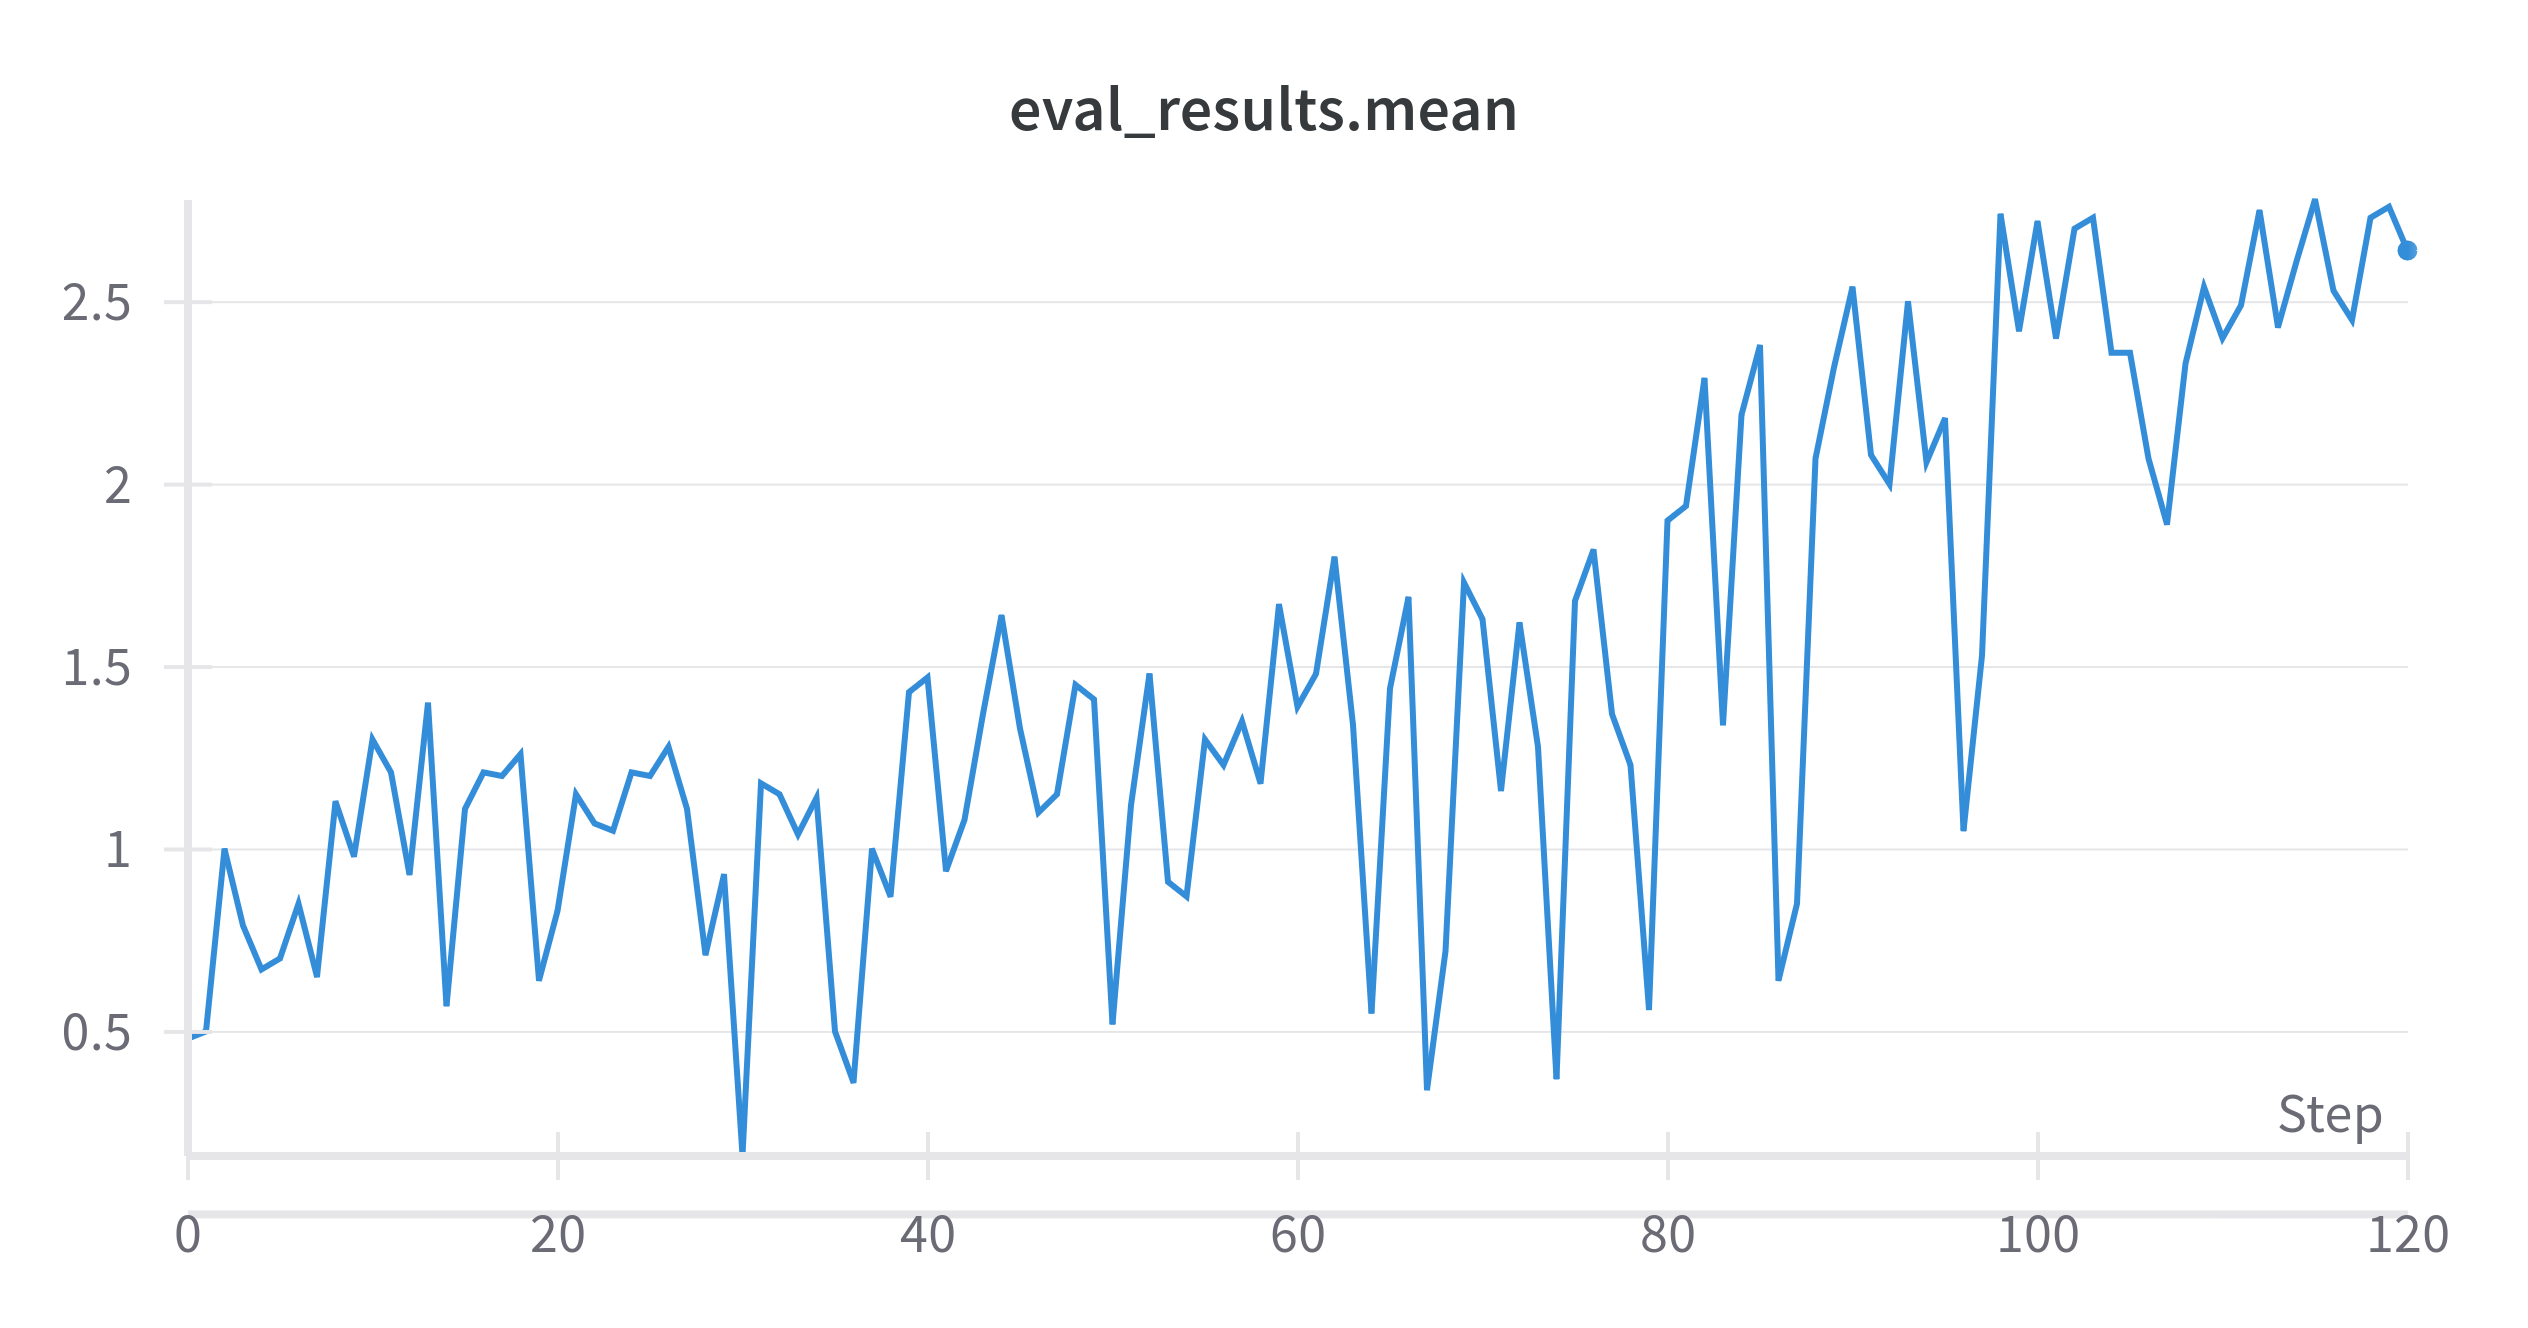
\includegraphics[width=\linewidth]{results/SAD-3-mean.png}
    \caption{
      Training curve for SAD-3 Agent
    }
    \Description{Training curve for SAD-3 Agent}
    \label{fig:sad3mean}
  \end{figure*}

  \begin{figure*}[h]
    \centering
    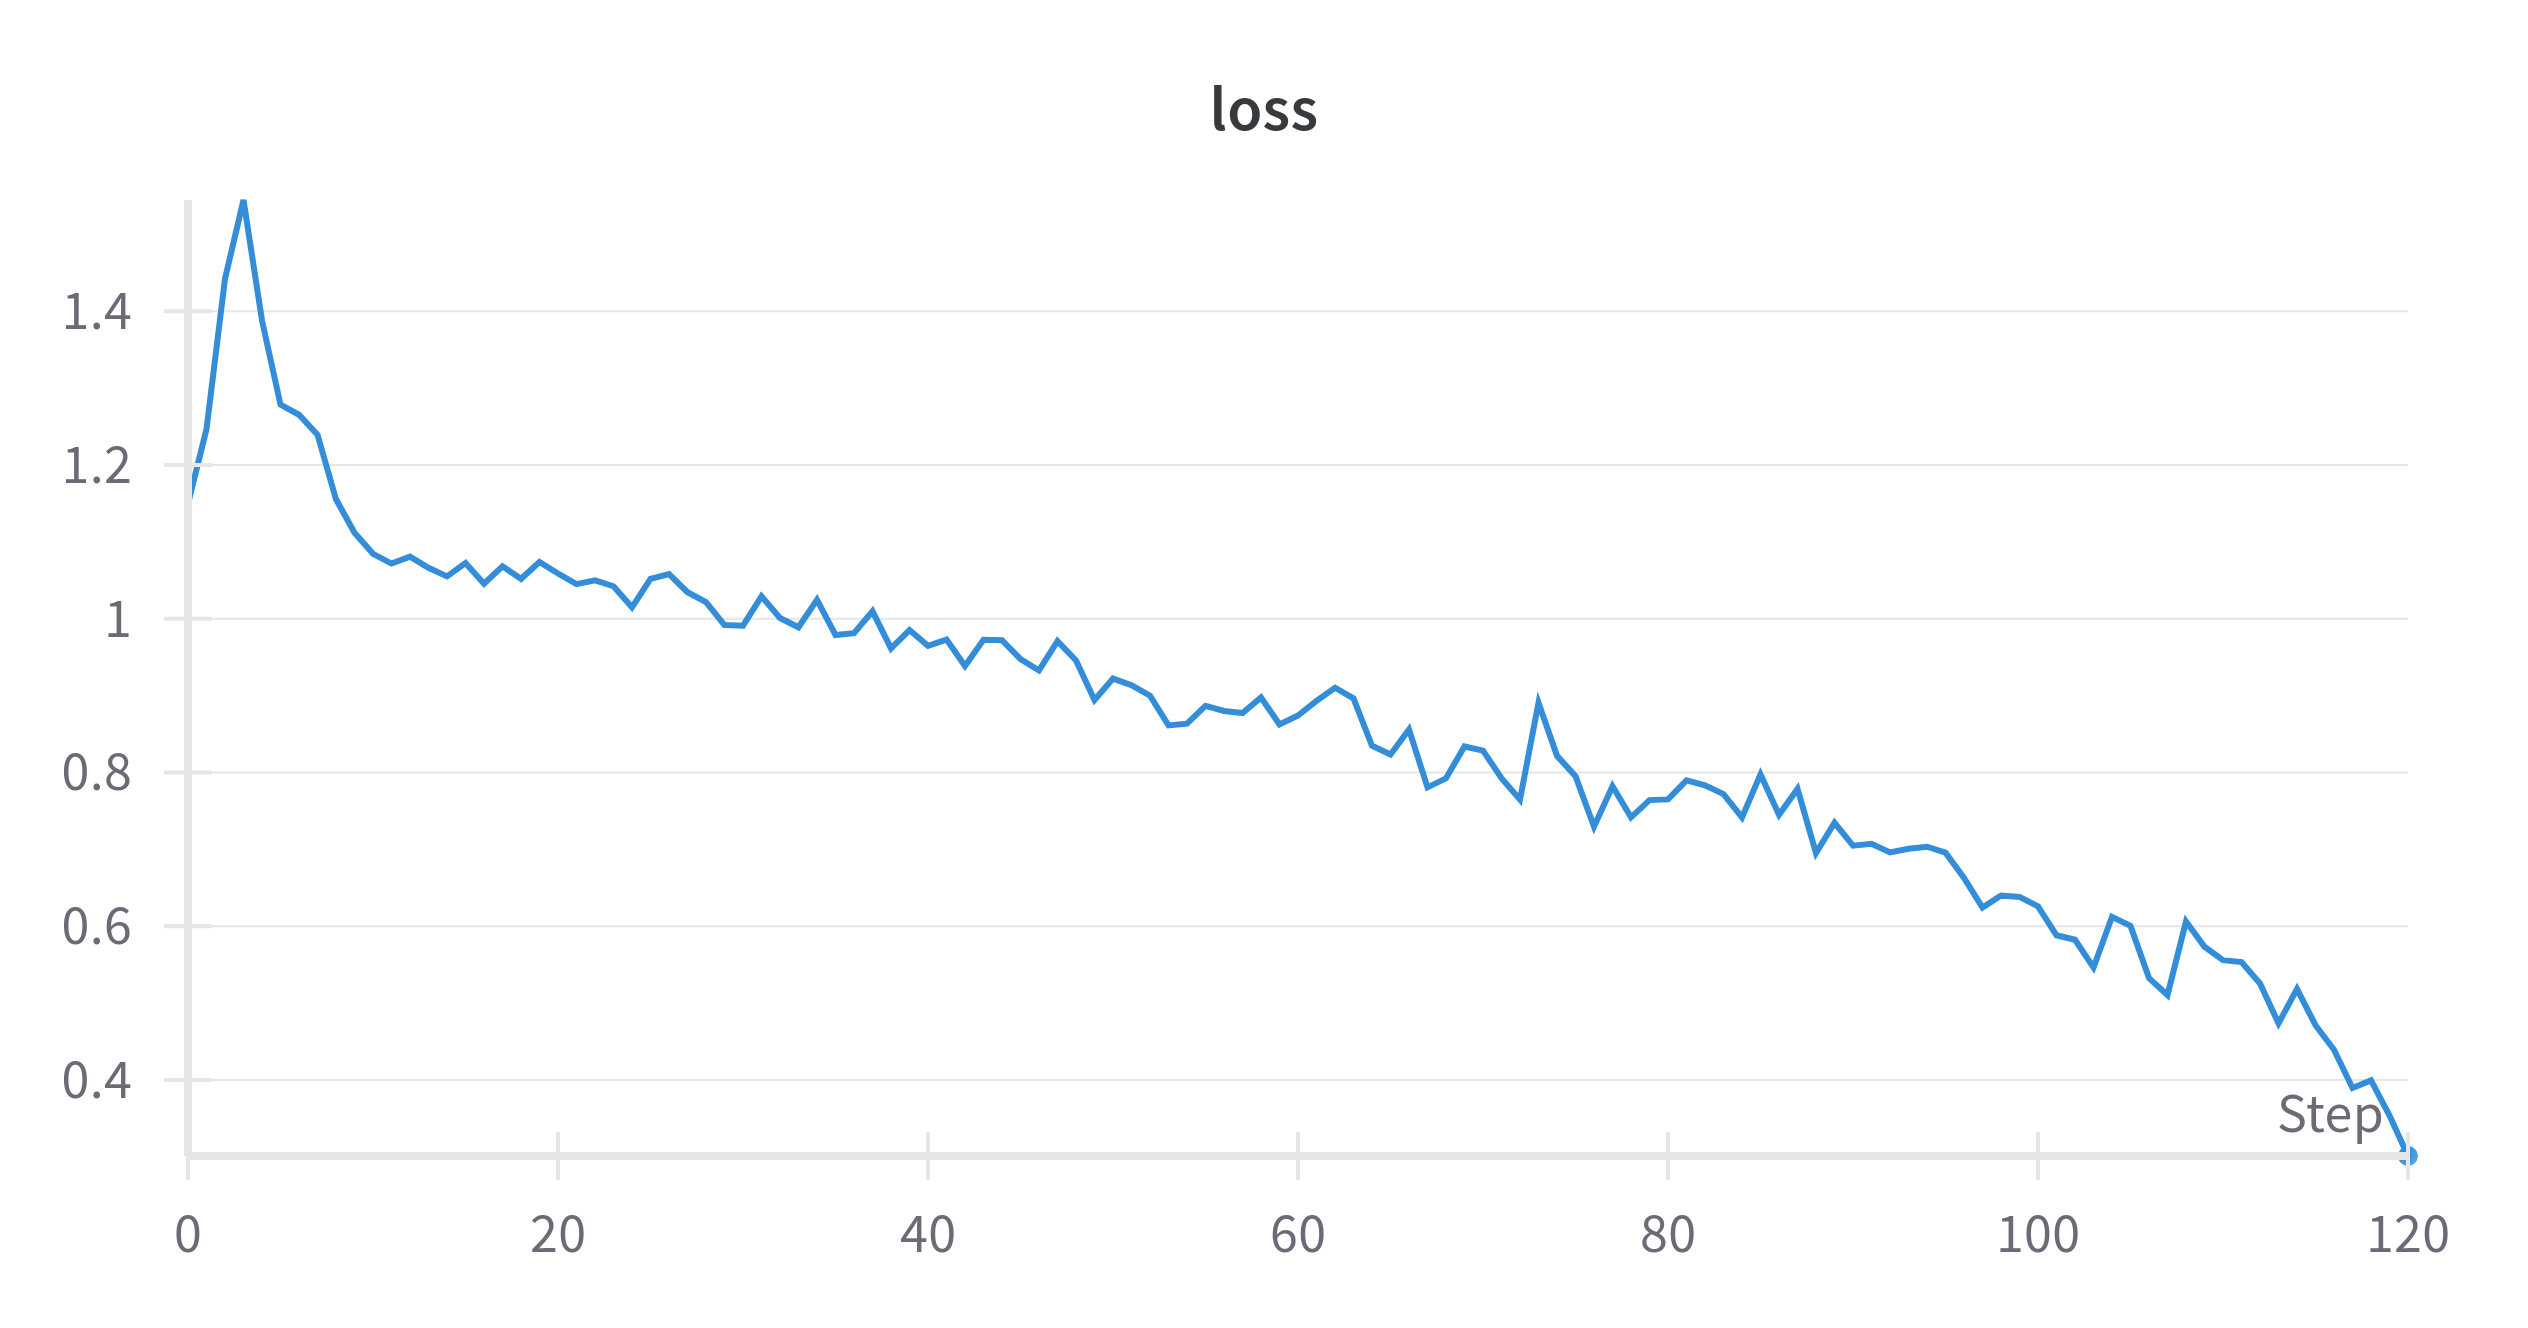
\includegraphics[width=\linewidth]{results/SAD-3-loss.png}
    \caption{
        Loss curve for SAD-3 Agent
    }
    \Description{Loss curve for SAD-3 Agent}
    \label{fig:sad3loss}
  \end{figure*}